\documentclass{book}
\usepackage[utf8]{inputenc}
\usepackage[francais]{babel}
\usepackage{titlesec}

\title{Optique des faisceaux Gaussiens}
\author{
  JÀÁJ AxxA\\
  \and
  Ema Gresal
}
\date{Décembre 2020}

\usepackage{natbib}
\usepackage{graphicx}
\usepackage{xcolor, soul}  
\usepackage{mdframed}
\usepackage{caption}
\usepackage{amsmath}
\usepackage{enumitem}

\definecolor{remarque1}{HTML}{0000A0}
\definecolor{remarque2}{HTML}{68B7FF}
\definecolor{definition1}{HTML}{8B0000}
\definecolor{definition2}{HTML}{FFC616}
\definecolor{attention1}{HTML}{FF0000}
\definecolor{attention2}{HTML}{FF8582}
\definecolor{exemple1}{HTML}{006400}
\definecolor{exemple2}{HTML}{B0FF1D}
\definecolor{fondamental1}{HTML}{4F4F4F}
\definecolor{fondamental2}{HTML}{BCBCBC}
\definecolor{complement1}{HTML}{0000A0}
\definecolor{complement2}{HTML}{68B7FF}

\newcommand{\sectionbreak}{\clearpage}
\newcommand{\subsectionbreak}{\clearpage}
\begin{document}

\maketitle
\chapter{Cours}
\section{Les résonateurs ouverts}
\subsection{Introduction}
 Les lasers sont par nature des résonateurs optiques. Ils sont principalement constitués de trois éléments essentiels :
\begin{itemize}
    \item Un milieu amplificateur de lumière
    \item Un système de pompage
    \item Une cavité résonante
\end{itemize}
\paragraph{}
Les deux premiers points sont traités en détail dans une autre partie du cours (Grain «lasers et applications»). L'objectif de ce cours est de traiter le troisième point, à savoir d'expliquer comment agit une cavité résonante placée autour d'un milieu amplificateur et quelles sont les propriétés du rayonnement laser liées à la présence de cette cavité. 

\subsection{Intérêt et description des résonateurs ouverts}
\paragraph{Introduction}

Le rôle de la cavité laser est de permettre l'amplification répétée de l'onde optique grâce à un système réfléchissant (la plupart du temps des miroirs). C'est aussi la cavité qui permet, via ses pertes (un des miroirs utilisé n'est que partiellement réfléchissant), d'extraire le faisceau laser utile. Enfin la géométrie de la cavité détermine en grande partie les caractéristiques spatiales et spectrales du rayonnement laser émis.

\paragraph{Pourquoi un résonateur ouvert ?}
Le résonateur le plus simple que l'on puisse imaginer est une boite parallélépipédique (fermée, donc) dont toutes les parois sont métallisées. Cette cavité possède un certain nombre de modes susceptibles d'osciller, et ces modes sont définis par les conditions aux limites sur les parois pour les vecteurs d'ondes (un mode est associé à un vecteur d'onde $\vec k_{mnq}$ avec $k_x = m \frac \pi a, k_y = n \frac \pi b, k_z = q \frac \pi d$ où $a, b, d$ sont les dimensions du parallélépipède).

Si on insère un milieu amplificateur dans une telle cavité, les modes vont se mettre à osciller et on aura amplification. Cependant, pour que l'onde produite soit cohérente, il faut que le nombre de modes susceptibles d'osciller, c'est à dire compris dans la bande spectrale d'amplification du milieu amplificateur, soit faible.

Si on calcule le nombre de modes dans cette bande de fréquence $\Delta \nu$, on trouve qu'il est proportionnel au volume de la cavité et inversement proportionnel à la longueur d'onde au carré. Numériquement, si la longueur d'onde vaut 10 cm (domaine des micro-ondes), alors une dizaine de modes sont susceptibles d'osciller dans une bande de 1 GHz et une cavité de dimensions raisonnables (10 cm de côté). Par contre, si la longueur d'onde appartient au domaine optique (par exemple 1 µm), alors on trouve pour cette cavité environ $10^{11}$ modes dans la même bande spectrale.

C'est pour cela que de tels résonateurs sont très bien adaptés pour réaliser des MASERS (Microwave Amplification by Stimulated Emission of Radiation) mais ne sont pas utilisables avec de la lumière visible : un trop grand nombre de modes vont osciller simultanément, ou, en d'autres termes, la taille de la cavité nécessaire pour obtenir un fonctionnement quasi-monomode est micrométrique.

\textbf{\color{remarque1}Remarque :}  
\begin{mdframed}[linecolor=remarque1, backgroundcolor=remarque2]
Avec la technologie actuelle, ce type de micro-cavité est réalisable – ce qui n'était pas le cas en 1960 – néanmoins, le milieu amplificateur est dans ce cas trop petit pour espérer réaliser des sources puissantes
\end{mdframed}

Il est donc nécessaire de modifier la géométrie du résonateur : l'idée proposée et développée, entre autre par Schallow et Townes dans les années 50, consiste à utiliser un résonateur quasi-linéaire où une seule direction d'oscillation est permise : c'est le résonateur ouvert, constitué dans sa forme la plus simple de deux miroirs face à face dans une configuration d'interféromètre de Fabry-Pérot.

En première approche, les modes d'un tel résonateurs sont similaires à ceux décrits pour la cavité fermée si on fait l'hypothèse que $d\gg a, b$. Une telle structure réduit considérablement le nombre de modes susceptibles d'osciller, comme on s'en rend compte avec le Fabry-Pérot : tous les rayons qui présentent un angle trop important par rapport à l'axe de la cavité vont rapidement sortir de cette dernière. Dans le cas du Fabry-Pérot, néanmoins, le moindre défaut de parallélisme va faire sortir tout faisceau de la cavité après quelques aller-retours seulement. Pour qu'un laser fonctionne efficacement, et que la cavité joue son rôle de filtre spatial et spectral, il faut que certains rayons restent dans la cavité assez longtemps : on a besoin de cavités stables, nous y reviendrons.

\paragraph{Description des résonateurs}

La cavité la plus simple pouvant être stable est la cavité linéaire constituée de deux miroirs face à face, de rayons de courbure $R_1$ et $R_2$, distants d'une distance $L$, et de diamètres respectifs $D_1$ et $D_2$ (voir figure 1). Dans ce type de cavité, une onde stationnaire est formée. Elle peut également contenir divers éléments optiques (des lentilles, des éléments polarisants, des composants actifs...) : on appelle « cavité passive » la cavité sans son milieu amplificateur, par opposition à la cavité active où le milieu amplificateur est présent.

{\centering
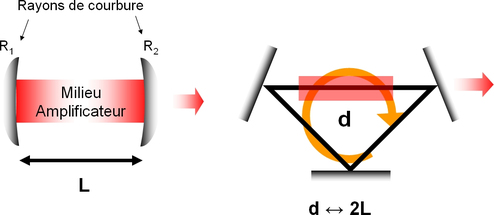
\includegraphics[scale=1.7]{images/fig01.jpg}
\captionof{figure}{ Cavité linéaire et cavité en anneau}
\par}

\textbf{\color{remarque1}Remarque :}  
\begin{mdframed}[linecolor=remarque1, backgroundcolor=remarque2]
Ce qui nous intéressera par la suite est le chemin optique [d] parcouru par la lumière lors d'un aller-retour dans la cavité, Ce chemin optique est défini comme le produit de la distance parcourue par l'indice de réfraction rencontré par la lumière.
\end{mdframed}
\textbf{\color{remarque1}Remarque :}  
\begin{mdframed}[linecolor=remarque1, backgroundcolor=remarque2]
Un autre type de cavité répandu est la cavité en anneau (voir figure 1.1), où la lumière ne revient pas sur elle-même mais forme une onde progressive. Dans ce cours, on se limitera en général à la cavité linéaire, mais les raisonnements et les méthodes utilisés sont valables pour tout résonateur.
\end{mdframed}*

\subsection{Modes spectraux et modes longitudinaux}

On peut définir les modes d'un résonateur ouvert en utilisant les expressions bien connues pour les résonateurs fermés : dans le cas du parallélépipède défini par les longueurs de ses trois côtés $a, b, d$, les fréquences $\nu_{mnq}$ sont données par $$\nu_{mnq} = \frac c 2 \sqrt{\left( \frac m a \right) ^2 + \left(
            \frac n b \right) ^2 + \left( \frac q d \right) ^2}$$
où $c$ est la vitesse de la lumière dans le vide.

Dans le cas d'un résonateur ouvert, $d\gg (a,b)$
et en prenant $a=b$ pour simplifier l'expression , on obtient $$\nu_{mnq} = \frac {qc}{2d} \sqrt{1+\frac {n^2 + m^2}{a^2} \frac{d^2}{q^2} }$$
ou encore après développement limité $$\nu_{mnq} \approx q \frac {c}{2d} + (m^2 + n^2) \frac{cd}{4qa^2}$$

On a ainsi une expression des fréquences des modes $TEM_{mnq}$.

Les modes longitudinaux sont les modes $TEM_{00q}$. Leur fréquences valent $\nu_q = q \frac c {2d}$ et on les appellent aussi parfois « modes spectraux » (voir figure 2.2).

{\centering
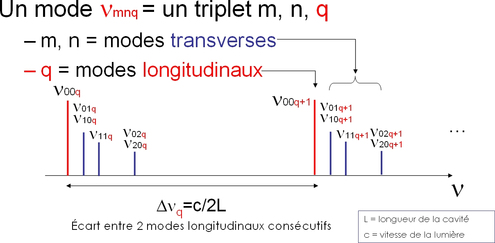
\includegraphics[scale=1.7]{images/fig02.jpg}
\captionof{figure}{ Modes longitudinaux et transverses dans une cavité résonante.}
\par}

Deux modes longitudinaux sont donc séparés de $\Delta \nu_q = \frac c {2d}$ soit pour $d$=10 cm un écart fréquentiel de 1,5 Ghz.

\textbf{\color{definition1}Définition :}  
\begin{mdframed}[linecolor=definition1, backgroundcolor=definition2]
Lorsqu'on parlera d'un laser « monomode longitudinal », on fera référence à un laser ayant une fréquence bien définie ($q$ fixé). Un seul mode longitudinal sera autorisé à osciller, ce qui conférera au susnommé laser une grande pureté spectrale ainsi qu'une longueur de cohérence importante
\end{mdframed}

Les modes transverses sont les modes $TEM_{mnq}$ avec $m$ et/ou $n$ différents de zéro (et presque toujours inférieurs à 10, rappelons que c'est le but du résonateur ouvert d'avoir un nombre de mode réduit).

\textbf{\color{definition1}Définition :}  
\begin{mdframed}[linecolor=definition1, backgroundcolor=definition2]
Un laser est dit « monomode transverse » lorsque seuls les modes $TEM_{00q}$ lasent.
\end{mdframed}


L'intervalle spectral entre deux modes transverses de $n$ et $q$ fixés vaut $$\delta\nu_m =
            (2m+1)\frac{cd}{4qa^2}$$ 
La répartition spectrale des modes longitudinaux et des premiers modes transverses est donnée sur la figure 2. On note que les modes $m^2+n^2=constante$ sont dégénérés.

\textbf{\color{remarque1}Remarque :}  
\begin{mdframed}[linecolor=remarque1, backgroundcolor=remarque2]
Cette analyse est valable dans le cadre d'une approche «ondes planes». On verra par la suite que les expressions sont différentes pour des faisceaux gaussiens.
\end{mdframed}

\textbf{\color{exemple1}Exemple :}  
\begin{mdframed}[linecolor=exemple1, backgroundcolor=exemple2]

{\centering
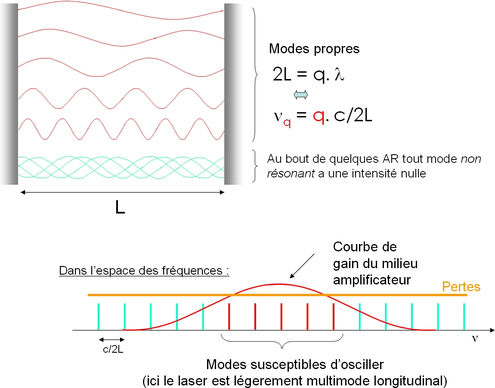
\includegraphics[scale=1.7]{images/fig03.jpg}
\captionof{figure}{ Répartition spectrale des modes longitudinaux d'un laser}
\par}

Quelle est la largeur spectrale d'un laser faiblement multimode ? Et d'un laser monomode ?

Considérons une cavité de 15 cm de longueur optique. L'écart entre deux modes consécutifs est $\frac c {2L}$, soit ici 1 GHz. Si on considère que 5 modes sont susceptibles d'osciller (cas de la figure 1.3) on obtient une largeur spectrale en fréquence de 5 GHz, ou encore en passant en longueur d'onde de 17 pm. C'est bien inférieur à la résolution de la plupart des spectromètres : le laser apparaît monochromatique (même si en toute rigueur il n'est pas monomode).

Pour certaines applications (métrologie...) on a besoin de lasers plus fins spectralement : on peut alors forcer le comportement monomode (par exemple en diminuant les pertes pour un seul des modes susceptibles d'osciller). La largeur spectrale obtenue est alors la largeur naturelle d'une seule raie laser, qui dépend beaucoup du type de milieu laser employé (gaz, solide...), et dont l'ordre de grandeur peut varier de quelques Hz au MHz et plus.
\end{mdframed}

\section{Stabilité des cavités lasers}
\subsection{Introduction}
Nous allons décrire ici une approche simple fondée sur l'optique géométrique avant d'aborder la description plus exacte basée sur les équations de Maxwell (voir paragraphe sur les faisceaux gaussiens). 

Nous considérerons des cavités passives, les cavités réelles pouvant en général au premier ordre y être ramenées (en modélisant par exemple les effets thermiques dus à l'échauffement - créé par l'absorption de la pompe - dans le milieu amplificateur par une simple lentille). Comme de coutume en optique géométrique, la propagation de la lumière sera donc décrite en termes de « rayons » définis en chaque point d'une onde comme la normale au front d'onde. C'est aussi la direction de propagation de l'énergie (colinéaire au vecteur de Poynting). Enfin on se limitera aux systèmes centrés à symétrie axiale : la plupart des cavités réelles peuvent en première approximation s'y ramener. On travaillera avec des rayons paraxiaux, c'est à dire quasi-parallèles à l'axe optique $Oz$ de la cavité. On pourra travailler en projection dans le plan $yOz$, les raisonnements pouvant se répéter à l'identique dans $xOz$.

\subsection{Structure périodique des cavités lasers}
Considérons la cavité déjà décrite figure 1.1. Un rayon faisant des aller-retours dans cette cavité peut être « déplié » selon $Oz$. Autrement dit, le trajet de la lumière peut être représenté comme une succession d'allers simples de $M_1$ à $M_2$ puis de $M_2$ à $M_1$ etc. Il suffit pour cela de remplacer les miroirs de rayons de courbure $R_i$ par des lentilles de distance focale $f_i=\frac {R_i} 2$ (voir cours d'optique géométrique). 

{\centering
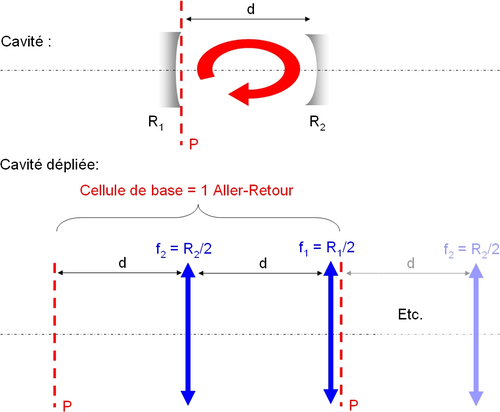
\includegraphics[scale=1.7]{images/fig04.jpg}
\captionof{figure}{ Dépliement d'une cavité à deux miroirs}
\par}

On peut ainsi comprendre intuitivement la notion de stabilité d'une cavité : si en traversant la séquence périodique de lentilles le rayon reste confiné près de l'axe, la cavité sera stable. Au contraire, s'il diverge, la cavité sera instable.

\subsection{Matrices de transfert et loi ABCD}
\paragraph{Introduction}
Même s'il est possible d'obtenir un laser avec des cavités instables dans certains cas bien particuliers (voir plus loin), il est en général préférable d'avoir une cavité stable. L'étude théorique de la stabilité est indispensable pour dimensionner la cavité (choix des rayons de courbure, des distances) avant de commencer à la construire. 
\paragraph{Les matrices de transfert}
L'étude de la stabilité de la cavité sera faite en utilisant la notion de matrice de transfert (ou matrices ABCD).

Le principe de cette méthode est d'associer à chaque élément optique au sens large (simple propagation dans un milieu donné, lentille, miroir...) une matrice 2x2 spécifique. On pourra ainsi déterminer les caractéristiques liées à la propagation par simple multiplication des matrices élémentaires.

Considérons une propagation dans le plan $yOz$, l'axe $z$ étant celui de la cavité. Dans ce plan, un rayon donné est caractérisé par son ordonnée de départ $h$ et par la pente $\theta$ de la droite qui supporte le rayon paraxial (voir figure 1.5). 

{\centering
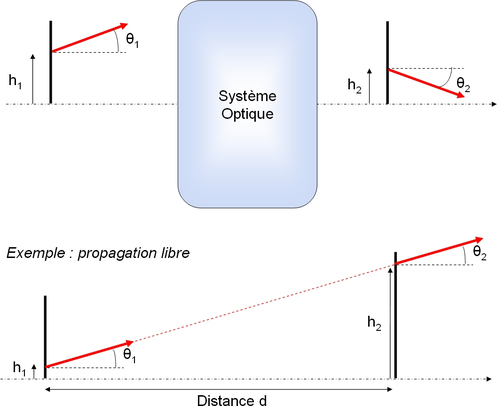
\includegraphics[scale=1.7]{images/fig05.jpg}
\captionof{figure}{ Définition des paramètres}
\par}

Dans les conditions de Gauss, les relations entre $(h_1 , \theta_1)$ avant la traversée d'un système optique donné et $(h_2 , \theta_2)$ après cette traversée sont linéaires et peuvent s'écrire sous forme matricielle : $$\begin{pmatrix}
            h_2 \\
            \theta_2 \\
            \end{pmatrix} = 
            \begin{pmatrix}
            A & B \\
            C & D \\
            \end{pmatrix} 
            \begin{pmatrix}
            h_1 \\
            \theta_1 \\
            \end{pmatrix}$$
où les termes diagonaux sont sans dimension, B et C ayant respectivement les dimensions d'une longueur et de l'inverse d'une longueur. 

La matrice $T = \begin{pmatrix}
            A & B \\
            C & D \\
            \end{pmatrix}$ caractérise complètement le système optique traversé.

Nous allons maintenant déterminer les matrices ABCD pour quelques composants essentiels d'une cavité, et montrer comment obtenir la matrice ABCD du système complet à partir de ces composants élémentaires.

\begin{itemize}[label=\textbullet, font=\LARGE \color{blue}]
    \item Propagation sur une distance $d$ :

$T = \begin{pmatrix}
            1 & d \\
            0 & 1 \\
            \end{pmatrix}$, la démonstration est évidente (voir figure 1.5) :

$h_2=h_1 + d \theta_2$ et $\theta_2 =\theta_1$ (les rayons étant paraxiaux, on assimile l'angle à sa tangente).

Or en développant l'expression matricielle ci-dessus: $\begin{matrix}
            h_2=Ah_1+B\theta_1 \\
            \theta_2 = Ch_1 +D\theta_1 \\
            \end{matrix}$

On en déduit par identification termes à termes : $A =1, B=d, C=0, D=1$.

Nous ne démontrerons pas les autres relations (le raisonnement est exactement le même) : cela pourra être fait sous forme d'exercice.
    \item Propagation sur une distance d dans un milieu d'indice $n$:$$T = \begin{pmatrix}
            1 & \frac d n \\
            0 & 1 \\
            \end{pmatrix}$$

    \item Dioptre plan entre deux milieux d'indices $n_1$ et $n_2$:$$T = \begin{pmatrix}
            1 &0 \\
            0 & {\frac{n_1}{n_2}} \\
            \end{pmatrix}$$

    \item Lentille mince de distance focale $f$:$$T = \begin{pmatrix}
            1 & 0 \\
            -\frac 1 f & 1 \\
            \end{pmatrix}$$

    \item Miroir concave ou convexe de courbure $R$:$$T = \begin{pmatrix}
            1 & 0 \\
            {-\frac{2}{R}} & 1 \\
            \end{pmatrix}$$
\end{itemize}

On retrouve bien sûr l'équivalence miroir-lentille avec $R=2f$ (voir plus haut).

\textbf{\color{attention1}Attention :}  
\begin{mdframed}[linecolor=attention1, backgroundcolor=attention2]

De manière générale, pour $N$ systèmes optiques successifs $S_i (i=1,2,...,N)$ ayant chacun une matrice $T_i$, la matrice de l'ensemble est le produit des matrices dans l'ordre inverse : $T_{systeme}=T_N...T_i...T_3T_2T_1$

Attention, en général les matrices ne commutent pas et l'ordre doit être strictement conservé.

La matrice $T$ est unitaire (son déterminant vaut 1), sauf dans le cas (rare) où le milieu de départ et le milieu d'arrivé ont des indices différents.

On verra par la suite que cette méthode matricielle s'applique non seulement en optique géométrique mais également pour les faisceaux gaussiens.
\end{mdframed}

\textbf{\color{remarque1}Remarque :}  
\begin{mdframed}[linecolor=remarque1, backgroundcolor=remarque2]

Il arrive souvent que des systèmes astigmates soient introduits dans les cavités lasers (miroirs sphériques hors d'axe, lames à incidence de Brewster, lentilles cylindriques, prismes...). Dans ce cas, il existe un comportement différent suivant les deux directions orthogonales. Il faut alors distinguer les matrices ABCD dans la direction $x$ et celles dans la direction $y$.
\end{mdframed}
\paragraph{La loi ABCD}

Elle permet de décrire la propagation d'une onde sphérique dans un système optique.

Considérons une onde sphérique issue d'un point $O_1$, avec un rayon de courbure $R_1$ à l'entrée d'un système optique donné et convergeant en un point $O_2$ avec un rayon de courbure $R_2$ à la sortie de ce système. On prendra comme convention : $R>0$ lorsque l'onde diverge et $R<0$ lorsque l'onde converge.

On a dans ces conditions $R_1 \approx \frac {h_1}{\theta_1}$ et $R_2 \approx \frac {h_2}{\theta_2}$ (voir figure 1.6)

{\centering
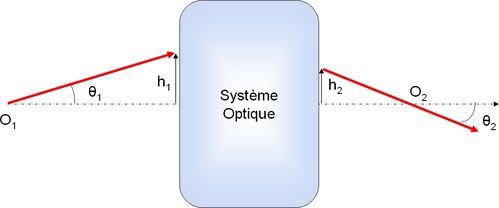
\includegraphics[scale=1.7]{images/fig06.jpg}
\captionof{figure}{ Paramètres pour la démonstration de la loi ABCD}
\par}

On peut donc déduire à partir de la définition de la matrice ABCD :

  $$R_2 = \frac{AR_1 + B}{CR_1 + D}$$
  
C'est la loi ABCD. \textbf{\color{red}Cette loi est très importante}, notamment parce qu'on la généralisera au cas des rayons de courbure complexes (voir plus loin le chapitre sur les faisceaux gaussiens). 

\subsection{Stabilité d'une cavité}
\paragraph{Étude générale}
 Considérons une cavité représentée par une structure périodique d'éléments optiques. La matrice de transfert de l'ensemble est $T = \begin{pmatrix}
            A & B \\
            C & D \\
            \end{pmatrix}$ 

Pour $n$ périodes, soit $n$ aller-retours dans le cas d'une cavité linéaire, la matrice de transfert est $T^n$. Si on note $p_0 = \begin{pmatrix}h_0 \\ \theta_0 \end{pmatrix}$ le vecteur représentant un rayon à l'entrée de la séquence, et $p_n = \begin{pmatrix}h_n \\ \theta_n \end{pmatrix}$ le vecteur à la sortie, on a $p_n = T^n p_0$. 

La matrice $T$ est diagonalisable, et si on note $P$ la matrice de passage unitaire et $x_{1,2 }$ les deux valeurs propres de $T$, on a $T=P \begin{pmatrix} x_1 & 0 \\ 0 & x_2 \end{pmatrix} P^{-1}$.

On en déduit donc que $$p_n=P \begin{pmatrix} x_1^n & 0 \\ 0 & x_2^n \end{pmatrix} P^{-1}p_0$$.

Pour que la cavité soit stable, il faut que les rayons restent au voisinage de l'axe optique au cours de la propagation à travers les $n$ éléments quand $n$ tend vers l'infini. Autrement dit, il faut que $p_n$ soit borné supérieurement, ou encore que $\lvert {x_1} \rvert \leq 1$ et $\lvert{x_2}\rvert \leq 1$.

Par ailleurs, les valeurs propres $x_1$ et $x_2$ de $T$ obéissent aux relations suivantes (voir cours d'algèbre linéaire):

$$x_1x_2 = \lvert T \rvert = 1\ (T\ est\ unitaire)$$

$$x_1+x_2=Trace(T)=A+D$$

Comme $x_1$ est à priori un complexe, on pose $x_1 = \lvert x_1 \rvert e^{i\phi}$ et par suite $x_2 = \lvert x_1 \rvert ^1 e^{i\phi}$.

Donc comme $\lvert {x_1} \rvert \leq 1$ et $\lvert {x_2} \rvert \leq 1$, on a forcément $\lvert {x_1}
            \rvert = \lvert{x_2}\rvert = 1$. Ensuite, la relation faisant intervenir la trace $T$ de conduit à $2
            cos(\phi)=A+D$. 

On en déduit \textbf{\color{red}la condition de stabilité applicable à toute cavité} :

$$-1\leq
            \frac{A+D} 2 \leq 1$$

ou encore

$$0 \leq \frac {A+D+2} 4 \leq 1$$

\textbf{\color{definition1}Définition :}  
\begin{mdframed}[linecolor=definition1, backgroundcolor=definition2]
Une cavité est stable quand les coefficients de sa matrice vérifient la condition de stabilité énoncée ci-dessus. 
\end{mdframed}

\paragraph{Exemple d'application}

Prenons une cavité linéaire simple de longueur $d$ à deux miroirs de rayons de courbures $R_1$ et $R_2$, équivalente à une séquence périodique de deux lentilles minces de focales $f_1 = \frac {R_1} 2$ et
$f_2 = \frac{R_2}2$, séparées d'une distance $d$. 

 La matrice $T$ vaut (voir figure 4): 

$$T = \begin{pmatrix} 1 & 0 \\ \frac {-1}{f_1} & 1 \end{pmatrix}
            \begin{pmatrix} 1 & d \\ 0 & 1 \end{pmatrix} \begin{pmatrix} 1 & 0 \\ \frac {-1}{f_2} & 1 \end{pmatrix}
            \begin{pmatrix} 1 & d \\ 0 & 1 \end{pmatrix} = \begin{pmatrix} 1-\frac d {f_2} & d\left(2-\frac d
            {f_2}\right) \\ \frac {-1}{f_1}-\frac {1}{f_2}+\frac {d}{f_1f_2} & \left(1-\frac d {f_1}\right)\left(1-\frac
            d {f_2}\right) - \frac d {f_1} \end{pmatrix}$$

On montre alors facilement que

$$\frac{A+D+2}4=\left(1-\frac d{R_1}\right)\left(1-\frac d{R_2}\right)$$

On a l'habitude de poser $g_i=1-\frac d {R_i}$ et on obtient \textbf{\color{red}la condition de stabilité de la cavité pour une cavité linéaire à deux miroirs} :

$$0\leq g_1g_2 \leq 1$$

On visualise classiquement cette condition de stabilité sur un diagramme représentant l'espace $g_2(g_1)$, c'est à dire en prenant $g_2$ comme axe des ordonnées et $g_1$ comme axe des abscisses (figure 7).

{\centering
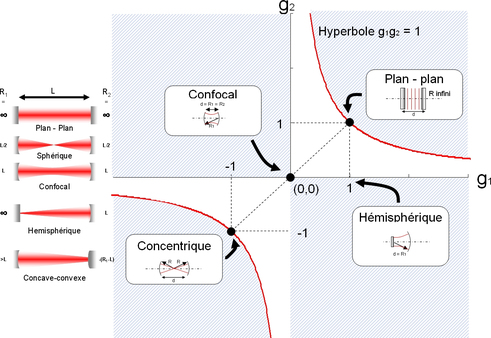
\includegraphics[scale=1.7]{images/fig07.jpg}
\captionof{figure}{ Conditions de stabilité pour une cavité linéaire à deux miroirs et exemple de cavités classiques.}
\par}

 La condition de stabilité est alors représentée par deux hyperboles, et les zones d'instabilité sont hachurées sur la figure.

Quelques cas particuliers sont remarquables :
\begin{itemize}
    \item Sur l'hyperbole $g_1g_2=1$: on a alors $d=R_1+R_2$, ce sont les cavités dites concentriques.
    \item Les droites $g_1=1$ et $g_2=1$ correspondent à des cavités où l'un des miroirs est plan (rayon de courbure infini). La cavité Fabry-Pérot (2 miroirs plans) est obtenue pour $g_1=g_2=1$.
    \item Pour $R_1 = R_2 = d\ (g_1 = g_2 = 0)$, on a une cavité dite « confocale ».
\end{itemize}

\textbf{\color{remarque1}Remarque :}  
\begin{mdframed}[linecolor=remarque1, backgroundcolor=remarque2]

Il existe une méthode graphique, dite « méthode des cercles de Deschamps », qui permet de savoir si une cavité à deux miroirs sphériques est stable : il suffit de vérifier que les deux cercles de diamètres $R_1$ et $R_2$ centrés sur les points focaux $F_1$ et $F_2$ se coupent (voir figure 8). Si c'est le cas, la cavité est stable (on peut vérifier que cela est une conséquence directe de la formule établie plus haut).

Les cercles de Deschamps permettent également d'avoir accès (voir figure 8) à la position du « waist » (intersection des cercles) et à la « longueur de Rayleigh » $Z_R$, deux paramètres qui seront définis dans la suite de ce cours.

{\centering
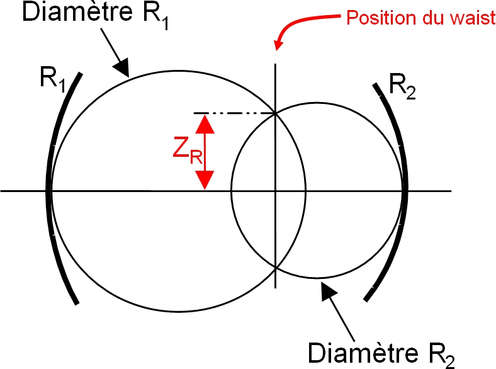
\includegraphics[scale=1.7]{images/fig08.jpg}
\captionof{figure}{ Cercles de Deschamps }
\par}

\end{mdframed}

Il n'est pas obligatoire de disposer d'une cavité stable pour obtenir un effet laser. Dans certains cas, lorsque le gain du milieu laser est suffisant pour permettre des pertes très élevées, les résonateurs instables présentent des avantages importants. C'est en particulier le cas des lasers de très haute puissance.

\paragraph{Cavités instables}

L'avantage principal de ces cavités est que le volume du mode dans la cavité peut être important, ce qui diminue la densité de puissance sur les miroirs (important pour les lasers de fortes puissances, où les seuils de dommage sont rapidement atteints). De plus, les modes transverses subissent de très fortes pertes, et ces cavités oscillent donc naturellement sur leur mode fondamental en général.

{\centering
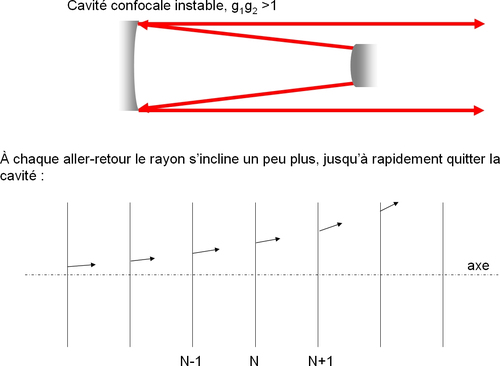
\includegraphics[scale=1.7]{images/fig09.jpg}
\captionof{figure}{ Exemple de cavité instable hémisphérique }
\par}

Ces cavités ne sont possibles qu'avec des milieux à très fort gain puisqu'un rayon donné ne fait que quelques passages dans le milieu amplificateur avant de s'échapper de la cavité. 

\section{Les faisceaux gaussiens}
\subsection{Équation d'onde paraxiale et onde sphérique}

Une onde électromagnétique se propageant dans un milieu homogène est soumise aux équations de Maxwell. On déduit classiquement de ces équations que l'onde se propageant en milieu isotrope doit vérifier l'équation de propagation suivante

$$\Delta \overrightarrow E-\frac 1{c^2}\frac{\partial ^2 \overrightarrow E}{\partial
            t^2}=0$$

Si on considère la propagation d'un rayonnement électromagnétique monochromatique de fréquence $\nu = \frac
            \omega {2\pi}$, on peut réécrire ces équations sous une forme différente et montrer que l'onde doit vérifier \textbf{\color{red}l'équation de Helmholtz}:
            
            $$\Delta
            E(x, y, z) + k^2E(x, y, z) = 0$$
            
où $k=\frac \omega c$ est le vecteur d'onde.

Cette équation admet en particulier pour solution bien connue l'onde sphérique divergente dont la forme peut s'écrire :

$$E(x, y, z) = \frac {E_0} r e^{-ikr}$$

au point d'observation situé à une distance $r$ du point source placé à l'origine du repère $(x,y,z)$.

Dans le cadre de l'approximation paraxiale, on considère que le champ s'est propagé suivant une direction privilégiée, celle de l'axe $z$, et l'observation s'effectue donc sur un point peu éloigné de cet axe. Dans ce cas on peut effectuer un développement limité sur la distance entre le point source et le point d'observation :

$$r=\sqrt{x^2+y^2+z^2}\approx z + \frac {x^2 + y^2}{2z}$$

Le champ électrique au point d'observation devient alors :

$$E_{paraxial}(x, y, z) = \frac {E_0} z e^{-ikz}e^{-ik \frac {x^2 + y^2}{2z}}$$

Il s'agit du champ d'une "onde sphérique paraxiale", qui n'est qu'une solution approchée de l'équation de Helmholtz où l'on reconnaît le facteur de propagation en $e^{-ikz}$ et le facteur de variation transverse d'amplitude :

$$\frac 1 z e^{-ik \frac {x^2 + y^2}{2z}}$$

D'un point de vue strictement mathématique, l'onde sphérique est solution de l'équation de propagation et du point de vue physique, l'onde sphérique paraxiale est une solution approchée convenable pour décrire la propagation des ondes dans un espace libre. Néanmoins, dans le cas qui nous occupe, à savoir les lasers, cette onde est une solution peu avantageuse car l'énergie se répandant dans tout l'espace, on doit diaphragmer le faisceau pour en isoler une portion proche de l'axe. On a donc des pertes importantes ce qui est incompatible avec l'émission laser.

En effet, la structure du champ électromagnétique à l'intérieur d'une cavité laser doit vérifier les conditions suivantes :
\begin{itemize}
    \item Satisfaire aux équations de Maxwell
    \item Le champ doit décroître lorsque l'on s'éloigne de l'axe de la cavité en raison de la taille finie des miroirs et du milieu à gain.
    \item Le front d'onde doit être adapté au rayon de courbure des miroirs (ce qui exclu les ondes planes)
\end{itemize}
Nous allons maintenant décrire les solutions adaptées aux résonateurs lasers. 

\subsection{Onde sphérique gaussienne}

 Nous allons introduire ici une généralisation des solutions mathématiques de l'équation de Helmholtz, dont nous détaillerons par la suite la signification physique.

Considérons les solutions de l'équation de Helmholtz correspondant à des faisceaux qui se propagent globalement selon $Oz$, avec des rayons paraxiaux.

La solution s'écrit de façon générale sous la forme suivante :

$$E(x, y, z) = \psi (x, y, z) e^{-ikz}$$

où $\psi (x, y, z)$ est une fonction complexe lentement variable qui représente les différences entre un faisceau laser et une onde plane homogène.

En remplaçant cette solution dans l'équation de Helmholtz et en faisant l'hypothèse que les variations de $\psi
            (x, y, z)$ dans la direction $Oz$ sont négligeables sur une distance de l'ordre de la longueur d'onde (soit $\lambda
            \lvert
            \frac {\partial \psi}{\partial z}\rvert \ll \lvert \psi \rvert$ et $\lambda \lvert \frac {\partial ^2
            \psi}{\partial z^2}\rvert \ll \lvert \frac {\partial \psi}{\partial z}\rvert$ ), on peut réécrire \textbf{\color{red}l'équation d'onde paraxiale} sous la forme :
            $$\frac {\partial ^2
            \psi}{\partial
            x^2}+\frac {\partial ^2 \psi}{\partial y^2} -2ik \frac {\partial \psi}{\partial z}=0$$
            
\textbf{\color{remarque1}Remarque :}  
\begin{mdframed}[linecolor=remarque1, backgroundcolor=remarque2]
On retrouve ici la forme de l'équation d'onde de Schrödinger pour une particule libre dans un espace à 2D $(x,y)$ avec le temps $t$ remplacé par $z$. 
\end{mdframed}

Les solutions de l'équation d'onde paraxiale sont connues. On peut ainsi vérifier facilement qu'une fonction (il en existe d'autres) de la forme :
$$\psi (x, y, z) = e^{-i\left(\Delta \phi (z) + \frac k {2q(z)}(x^2+y^2)\right)}$$

est solution, avec :
\begin{itemize}
    \item $\Delta\phi(z)$ est un déphasage complexe (déphasage réel et changement d'amplitude avec $z$).
    \item $q(z)$ représente un rayon de courbure complexe, ou encore la variation transverse de l'amplitude et la courbure du front d'onde.
\end{itemize}

Cette solution particulière, appelée \textbf{\color{red}« Mode fondamental Gaussien »}, est la plus importante en pratique dans les résonateurs lasers. Nous allons donc la traiter en détails par la suite.

En substituant l'expression de $\psi(x, y, z)$ dans l'équation d'onde paraxiale, on obtient que pour tout $(x,y)$:

$$\left( \frac {k^2}{q^2} (x^2+y^2) \left(\frac {dq}{dz} -1 \right) -2k \left( \frac{d\Delta\phi}{dz} +
            \frac i
            q\right)\right)\psi = 0$$

On en déduit que $q(z)$ et $\phi(z)$ doivent vérifier :

$$\frac{dq}{dz}=1 \Rightarrow q(z)=q_0+z\ avec\
            q_0=q(0)$$
$$\frac{d\Delta \phi}{dz}=-\frac i q \Rightarrow \Delta\phi(z)=-i\ ln\left(\frac{q_0+z}{q_0}\right)\ si\
            \Delta
            \phi(0)=0$$
            
De plus on pose $\frac 1 {q(z)}=\frac 1 {R(z)}-i\frac {\lambda}{\pi w^2(z)}$

On a alors
$$e^{-i\Delta\phi(z)} = \frac 1 {1 + \frac z {q_0}}=\frac 1 {1+\frac z {R_0}-\frac{i\lambda
            z}{\pi
            w_0^2}}$$
où les indices 0 indiquent les valeurs en $z=0$. Si on choisit à l'origine un rayon de courbure infini (c'est à dire une surface d'onde plane), on a $q_0=i\frac{\pi w_0^2}{\lambda}$. On peut alors facilement montrer que :

$$\frac 1 {q(z)}=\frac 1 {q_0 + z} = \frac {\frac{1}{q_0}} {1+\frac z {q_0}}= \frac 1 {1+\left(\frac
            {\lambda
            z}{\pi w_0^2}\right)^2}\left(\frac 1 z \left( \frac {\lambda z}{\pi w_0^2} \right)^2-i \frac \lambda {\pi
            w_0^2}
            \right)$$

En identifiant cette dernière relation avec $\frac 1 R -i \frac \lambda {\pi w^2(z)}$ on déduit:

$$R(z)=z+\frac{Z_R^2}{z}\ avec\ Z_R=\frac {\pi w_0^2} \lambda$$

$$w(z) = w_0\sqrt{1+\left(\frac z {Z_R}\right)}$$

D'autre part:

$$e^{-i\Delta \phi (z)}=\frac 1 {1-\frac {iz}{Z_R}}=\frac 1 {\sqrt{1+\left( \frac z
            {Z_R}\right)^2}}e^{i\zeta
            (z)} \ ou \ tan(\zeta (z))=\frac z {Z_R}$$

avec :
\begin{itemize}
 
    \item $\frac K {w(z)}$ est un facteur de normalisation
    \item la première exponentielle est le terme propagatif
    \item la seconde exponentielle est un déphasage dit « de Gouy »
    \item la troisième exponentielle peut être décomposée en un terme « onde sphérique » et un terme « gaussienne » en remplaçant $q$ par son expression en fonction de $R$:
    
    $$e^{-ik\frac {r^2}{2q}} = e^{-ik \frac {r^2}{2R}}e^{-\frac {r^2}{w^2}}$$
    
\end{itemize}

où on est passé en coordonnées cylindriques ($r^2=x^2 + y^2$)


\textbf{\color{fondamental1}Fondamental :}  
\begin{mdframed}[linecolor=fondamental1, backgroundcolor=fondamental2]

Finalement, en regroupant toutes ces expressions, on obtient la relation suivante, qui est l'expression fondamentale de l'onde sphérique gaussienne :
$$E(x, y, z)=K \frac 1 {w(z)} e^{-ik(z)} e^{i\zeta(z)} e^{-ik \frac {x^2+y^2}{2q} }$$

\end{mdframed}

C'est là qu'apparaît le profil transverse gaussien en tout point de l'onde considéré. Le profil d'intensité (proportionnelle au carré du champ) du faisceau gaussien sera donc (voir figure 10) :

$$I(r, z) = I_0(z)e^{\frac {-2r^2}{w^2(z)}}$$

{\centering
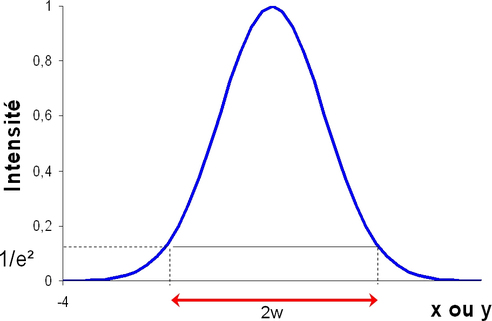
\includegraphics[scale=1.7]{images/fig10.jpg}
\captionof{figure}{ Profil d'intensité gaussien. }
\par}

\begin{itemize}
    \item $R(z) = z\left(1+\left(\frac{\pi w_0^2}{\lambda z}\right)^2\right)$ est le rayon de courbure du front d'onde qui coupe l'axe en $z$.
    \item $w(z) = w_0 \sqrt{1+\left(\frac{\lambda z}{\pi w_0^2}\right)^2}$ est une mesure de la décroissance – gaussienne - de l'amplitude du champ avec la distance à l'axe $z$ (voir figure 10). Le paramètre $w$ est la distance au bout de laquelle l'amplitude est égale à $\frac 1 e$ fois sa valeur sur l'axe ($\frac 1 {e^2}$ si on considère les intensités).
\end{itemize}


\textbf{\color{definition1}Définition :}  
\begin{mdframed}[linecolor=definition1, backgroundcolor=definition2]

Ce paramètre $w$ est minimal à l'origine $z=0$, où le rayon de courbure $R$ est infini. Sa valeur est alors notée $w_0$ et on parle du « waist » du faisceau (on dit parfois « col » en français).

\end{mdframed}


\textbf{\color{definition1}Définition :}  
\begin{mdframed}[linecolor=definition1, backgroundcolor=definition2]

$Z_R = \frac {\pi w_0^2}{\lambda}$ est appelée la longueur de Rayleigh et décrit la divergence du faisceau (voir plus loin).

\end{mdframed}


On rappel aussi que :
\begin{itemize}
    \item $q=q_0+z$ et $\frac 1 q = \frac 1 R -i \frac \lambda {\pi w^2}$
    \item Ce déphasage signifie que l'onde gaussienne est déphasée de $\zeta (z)$ sur l'axe $z$ par rapport à une onde plane de même longueur d'onde « partie » depuis l'origine $z=0$ au même instant. Ce déphasage sur l'axe spécifique à l'onde gaussienne tend vers $\frac \pi 2$ lorsque $z$ tend vers l'infini. Lorsque l'onde passe par $z=0$, elle subit un déphasage global de $\pi$
\end{itemize}

    .
\textbf{\color{definition1}Définition :}  
\begin{mdframed}[linecolor=definition1, backgroundcolor=definition2]

$tan(\zeta)=\frac {\lambda z}{\pi w_0^2}$ et $\zeta (z)$ est souvent appelé « déphasage de Gouy ». 

\end{mdframed}

\subsection{Propriétés des faisceaux gaussiens}

 La plupart des relations fondamentales liées aux faisceaux gaussiens ont été mathématiquement obtenues au paragraphe précédent. Nous allons maintenant voir leur signification physique.

Prenons comme précédemment l'origine au « waist » $w_0$, qui correspond à l'onde plane gaussienne de rayon de courbure infini. On a défini la longueur de Rayleigh par la relation $Z_R = \frac {\pi w_0^2}\lambda$.

On a également obtenu la loi d'évolution de $w$ en fonction de $z$:

$$w(z) = w_0 \sqrt{1+\left(\frac z {Z_R}\right)^2}$$

$w(z)$ est une hyperbole (on peut réécrire la relation précédente $\frac {w^2}{w_0^2}-\frac{z^2}{Z_R^2} = 1$).

\paragraph{Les principaux paramètres utiles}

Rappelons les principaux paramètres utiles et leur définitions :
\begin{itemize}
    \item $w(z)$ est la dimension (le rayon) de la tache laser dans un plan perpendiculaire à la propagation à une distance $z$ de l'origine. Plus précisément, c'est le rayon à $\frac 1 e$ du profil gaussien d'amplitude transverse dans le plan d'abscisse $z$(à $\frac 1 {e^2}$ si on considère le profil d'intensité : dans la formule ci-dessous, $I=\frac {I_0}{e^2}$ pour $r = w$).
    
    $$I(r, z) = I_0(z)e^{\frac{-2r^2}{w^2(z)}}$$
    
    \item Le faisceau « s'étale » transversalement au cours de la propagation, tandis que son amplitude sur l'axe diminue (conservation de l'énergie). Le profil reste toujours gaussien.
    \item La taille du faisceau à l'origine, $w_0$, est la taille minimale du faisceau qui diverge à partir de ce point (voir figure 11). On appelle \textbf{\color{red}« waist »}, ou encore « col » ou « taille », cette dimension minimale (NB : le waist désigne bien le rayon minimal du faisceau. Le diamètre est évidemment donné par $2w_0$)
    \item Au waist, on a vu que le front d'onde était localement plan (de rayon de courbure infini).
{\centering
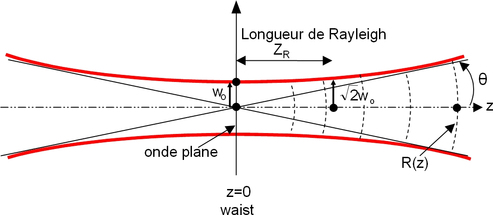
\includegraphics[scale=1.7]{images/fig11.jpg}
\captionof{figure}{ Propriétés d'un faisceau gaussien }
\par}
    \item La divergence du faisceau est mesurée par la limite pour $z$ tendant vers l'infini de $\frac w z$ : $\lim_{z \to \infty} \frac w z = \frac {w_0}{Z_R} = \frac \lambda {\pi w_0}=tan(\theta)$ soit pour une faible divergence $tan(\theta) = \frac \lambda {\pi w_0} \approx \theta$
    \item Les propriétés « gaussiennes » du faisceau laser s'expriment essentiellement à proximité du waist. En effet, lorsque $z$ tend vers l'infini, le rayon de courbure complexe s'identifie à $R$ et on retrouve une onde sphérique.
    \item La longueur de Rayleigh est la distance (comptée en partant du waist) au bout de laquelle la taille du faisceau a augmenté d'un facteur $\sqrt 2$ (ou encore que sa surface a doublé). C'est un paramètre important car il défini (un peu arbitrairement) la distance sur laquelle le faisceau laser garde une taille relativement constante (comprise entre $w_0$ et $w_0 \sqrt 2$) - voir figure 11.
\end{itemize}


\paragraph{Ordre de grandeur}

\textbf{\color{remarque1}Remarque :}  
\begin{mdframed}[linecolor=remarque1, backgroundcolor=remarque2]

Pour un faisceau laser focalisé «assez efficacement » $w_0$ = 10 µm, et une longueur d'onde de 1 µm, on trouve alors $Z_R$ = 314 µm et une divergence (demi-angle) de 1,8 degrés.

Si on prend un « gros waist » de 1 mm, on trouve alors $Z_R$ = 3,14 m et une divergence (demi-angle) de 0,018 degrés. On a alors un faisceau que l'on qualifie généralement de « collimaté ».

\end{mdframed}

\textbf{\color{fondamental1}Fondametal :}  
\begin{mdframed}[linecolor=fondamental1, backgroundcolor=fondamental2]

Plus un faisceau est gros, moins il diverge. En optique gaussienne, « collimater un faisceau » est équivalent à « obtenir un faisceau de grand waist ».

On observe l'évolution de la longueur de Rayleigh et de la divergence sur la figure 12 pour une longueur d'onde de 1 µm.

{\centering
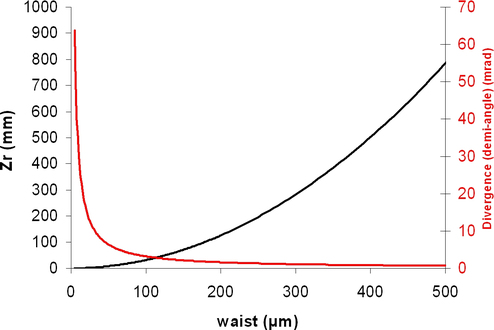
\includegraphics[scale=1.7]{images/fig12.jpg}
\captionof{figure}{ Evolution de la longueur de Rayleigh et de la divergence sur la figure 12 pour une longueur d'onde de 1 µm. }
\par}

\end{mdframed}

\paragraph{Autres relations utiles}

On peut déduire des relations précédentes d'autres équations utiles, comme par exemple :

$$w_0^2 = \frac {w^2}{1+\left(\frac{\pi w^2}{\lambda R}\right)^2}$$

et

$$z = \frac {R}{1+\left(\frac{\lambda R}{\pi w^2}\right)^2}$$

qui permettent de retrouver la taille du waist et sa position en connaissant $R$ et $w$. 

\subsection{Adaptation et focalisation des faisceaux gaussiens}

 La transformation subie par un faisceau gaussien lors de son passage dans une lentille est très souvent rencontrée expérimentalement. Lorsque l'on veut par exemple injecter un faisceau laser donné dans un autre laser pour le pomper, il importe que le faisceau soit convenablement «adapté» au résonateur du second laser.

Un faisceau gaussien est transformé en un autre faisceau gaussien par une lentille; nous allons maintenant voir comment.

En utilisant la loi ABCD (voir paragraphe sur "Les matrices de transfert et loi ABCD") appliquée à un système optique centré avec origines aux foyers, on peut trouver les relations entre les positions et les tailles d'un waist objet situé avant le système optique et celles du waist image obtenu après traversée du système.

Le « waist objet » $w_0$ est situé sur le plan repéré par l'abscisse $\sigma$ par rapport au foyer objet tandis que le « waist image » $w'_0$ est repéré par l'abscisse $\sigma '$ par rapport au foyer image (cf. figure 13).

\textbf{\color{remarque1}Remarque :}  
\begin{mdframed}[linecolor=remarque1, backgroundcolor=remarque2]

Il est en toute rigueur abusif de parler de waists objet et image puisqu'au sens strict les deux waists ne sont pas conjugués l'un de l'autre. En d'autres termes, le waist du faisceau image n'est pas l'image du waist du faisceau objet. On conservera néanmoins cette terminologie dans la suite.

\end{mdframed}

Le rayon de courbure complexe correspondant au waist objet est imaginaire pur et vaut:

$$q_0=i\frac{\pi w_0^2}{\lambda}$$

Les éléments de la matrice de transfert du système optique valent (à vérifier à titre d'exercice) :

$$A=\frac {-\sigma '}{f'};\ B=-f+\frac{\sigma \sigma '}{f'};\ C=\frac{-1}{f'};\ D=\frac \sigma {f'}$$

{\centering
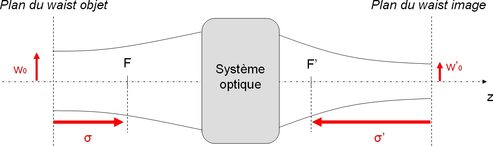
\includegraphics[scale=1.7]{images/fig13.jpg}
\captionof{figure}{ Relations de conjugaison pour les faisceaux gaussiens. }
\par}

En appliquant la loi ABCD et sachant que $q_0$ et $q_0'$ sont tous les deux des imaginaires purs, on trouve les relations suivantes :
$$\sigma \sigma ' = f f'-q_0q_0'$$
$$-\sigma q_0' = \sigma ' q_0$$
ou encore
$$\sigma \sigma ' = f f'-Z_RZ_R'$$
$$\frac {-\sigma}{Z_R} = \frac {\sigma '}{Z_R'}$$

Ces relations démontrent que la position du waist image dépend non seulement de la position du waist objet mais aussi de sa taille. De la même façon, la taille du waist image est fonction de la taille du waist objet et de sa position.
\begin{itemize}
    \item     Lorsque $\sigma \gg Z_R$, l'onde au niveau du foyer objet est quasi-sphérique (celui-ci est dans le champ lointain du faisceau). L'onde vue par la lentille semble donc être émise par un point source et on obtient : $\sigma \sigma ' = f f'$. On retrouve ici les relations conjugaison de Newton de l'optique géométrique.
    \item Un autre cas particulier est le cas $\sigma = 0$, c'est à dire que le waist objet est placé au foyer de la lentille. En optique géométrique, on s'attend à avoir alors un faisceau collimaté (rayons parallèles) en sortie de la lentille. En optique gaussienne, dans ce cas, on a aussi $\sigma ' = 0$ : le waist image est situé exactement sur le foyer image.
\end{itemize}

\textbf{\color{attention1}Attention :}  
\begin{mdframed}[linecolor=attention1, backgroundcolor=attention2]

On voit ici que les « relations de conjugaisons » gaussiennes diffèrent sensiblement de celles de l'optique géométrique dès lors que l'on se trouve à des distances comparables à $Z_R$. C'est dû au fait (voir remarque précédente) que ce qu'on appelle « relation de conjugaison » ici n'en est pas une au sens de l'optique géométrique.

\end{mdframed}

La relation de grandissement entre les waists est donnée dans ce cas par :

$$w_0' = \frac{\lambda f}{\pi w_0}$$

\textbf{\color{red}C'est une relation d'une grande importance pratique} car cette configuration se retrouve souvent expérimentalement. Elle permet très souvent d'obtenir un ordre de grandeur satisfaisant pour répondre à la question suivante : « quelle va être la taille du waist d'un faisceau laser après focalisation par une lentille de focale $f$ si je connais la taille du faisceau avant la lentille ? »

{\centering
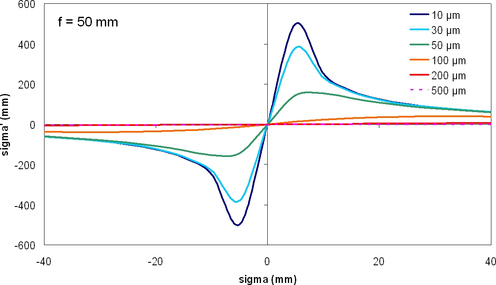
\includegraphics[scale=1.7]{images/fig14.jpg}
\captionof{figure}{ Evolution de la position du waist image en fonction de la position du waist objet(pour différentes tailles du waist objet) }
\par}

{\centering
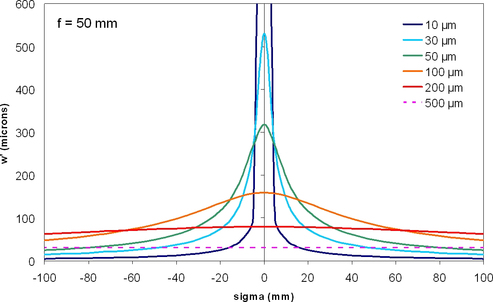
\includegraphics[scale=1.7]{images/fig15.jpg}
\captionof{figure}{ Evolution de la taille du waist image en fonction de la position du waist objet (pour différentes tailles du waist objet) }
\par}

En observant les figures 14 et 15 qui décrivent les équations ci-dessus, on peut faire quelques commentaires :

\begin{itemize}
    \item Sur la figure 14, lorsque la taille du waist objet est importante, on a $\sigma ' = 0$ quelque soit $\sigma$ : c'est le cas de l'optique géométrique où un faisceau collimaté (équivalent pour un faisceau gaussien à un faisceau de grand rayon $w$ comme on l'a souligné plus haut) vient se focaliser dans le plan focal image de la lentille. La position du waist objet a peu de sens ici puisque la distance de Rayleigh correspondant à un grand $w$ est très grande («collimation»).
    \item Lorsque la taille du waist objet est très petite (quasi ponctuelle), on se rapproche également de l'optique géométrique: on tend vers les asymptotes données par $\sigma \sigma ' = f^2$.
    \item En dehors des deux cas limite précédents, le comportement s'éloigne considérablement de l'optique géométrique: ainsi pour $w_0$=10 µm et $\sigma=0$(waist objet de petite taille au foyer objet de la lentille), on n'a pas une image à l'infini comme en optique géométrique mais une image située en $\sigma ' = 0$, c'est à dire sur le foyer image !
    \item Ce « paradoxe » n'en est pas un si on regarde la figure 15 : ainsi pour $w_0$=10 µm et $\sigma=0$ (waist objet au foyer objet de la lentille), le waist image est certes sur le foyer image, mais sa taille est très importante : le faisceau est donc quasiment collimaté et on retrouve un comportement « semblable à » celui de l'optique géométrique. 
\end{itemize}

\section{Mode fondamental Gaussien et cavité laser}
\subsection{Loi ABCD appliquée aux faisceaux gaussiens}

Un mode de cavité stable est caractérisé par le fait que le faisceau garde la même structure transverse et la même phase (modulo \(2 \pi\)) après un aller-retour dans la cavité (ou après un tour pour une cavité en anneau).
        

Plus précisément, le rayon de courbure complexe \(q(M)\) doit être conservé quelque soit le point \(M\) considéré. Autrement dit, si \(T(M)= \begin{pmatrix}
A & B \\
C & D \\
\end{pmatrix}\) est la matrice de transfert à partir du point \(M\) (attention, \(T(M)\) est
différente en fonction du
point \(M\) choisi), on doit avoir par application de la loi ABCD (voir paragraphe sur "les matrices de transfert et loi ABCD") et quelque soit \(M\) :
\[q(M) = \frac {Aq(M)+B}{Cq(M) + D}\]

\textbf{\color{red}C'est une condition complètement générale} qui s'applique à toute cavité
résonante. En identifiant les parties réelles et imaginaires de cette relation, on obtient deux équations qui définissent respectivement la géométrie du système (en particulier la position des waists) et les fréquences de résonance de la cavité.

La condition de stabilité découle également de la loi ABCD ci-dessus. On peut en effet la réécrire :
\[Cq^2+(D-A)q-B = 0\]

ou encore
\[B \left(\frac 1 q \right)^2 + (A-D) \frac 1 q -C=0\]

soit
\[\frac 1q=\frac1{2B}\left(D-A\pm\sqrt{(D-A)^2+4BC}\right)\]

qui vaut aussi
\[\frac 1R-i\frac\lambda{\pi w^2}\]

Pour que le faisceau existe, il faut que \(w\) soit fini, ou encore que \((D-A)^2+4BC\) soit strictement négatif (afin que la partie imaginaire de \(\frac 1q\) soit non nulle).

Comme la matrice $T$ est unitaire, on a $AD-BC = 1$ et la condition se réécrit donc: $(D+A)^2 < 4$ ou encore $-1 < \frac{A+D}2 < 1$ soit $0 < \frac{A+D+2}4 < 1$.

On retrouve la \textbf{\color{red}condition de stabilité} démontrée précédemment dans le cadre de l'optique géométrique, mais ici on remarque que l'inégalité est stricte : on exclut donc les cas limites où \(\lvert A+D\rvert =2\) qui représentent des cavités instables pour les faisceaux gaussiens.

La loi ABCD donne également les caractéristiques du faisceau gaussien au point \(M\):
\[R = \frac{2B}{D-A}\]

et

\[w^2 = \frac \lambda \pi \lvert B\rvert \sqrt{1-\left( \frac{A+D}2\right)^2}\]

On choisit souvent \(M\) à un waist du faisceau, c'est à dire à un endroit où le rayon de courbure \(R\) est infini. On constate alors que \(A=D\) dans la matrice \(T(M)\). Inversement, si \(A=D\) alors le point \(M\) est à un waist de la cavité.

\subsection{Cavité à deux miroirs}

Nous allons étudier plus en détail la cavité classique à deux miroirs sphériques de rayons de courbure \(R_1\) et \(R_2\) distants de \(d\).


\paragraph{Géométrie de la cavité}

Si un faisceau gaussien est un mode d'un tel résonateur, alors nécessairement son rayon de courbure est égal (en valeur absolue) au rayon de courbure des miroirs au niveau de ces derniers. C'est une condition indispensable pour assurer le retour sur lui-même du faisceau.

Si on appelle \(z_1\) et \(z_2\) les positions des miroirs \(M_1\) et \(M_2\) respectivement, on a donc \(R(z_1) = -R_1\) et \(R(z_2) = R_2\).

\textbf{\color{remarque1}Remarque :}  
\begin{mdframed}[linecolor=remarque1, backgroundcolor=remarque2]

Attention aux conventions de signe: ici on prend \(R>0\) pour une onde divergente et \(R<0\) pour une onde convergente.

\end{mdframed}


{\centering
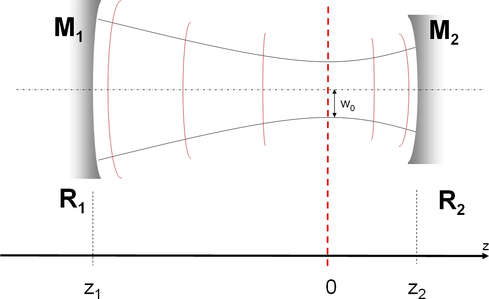
\includegraphics[scale=1.7]{images/fig16.jpg}
\captionof{figure}{ Géométrie de la cavité utilisée pour la démonstration}
\par}


Grâce à cette propriété, on peut déterminer la géométrie du mode dans la cavité sans passer par la loi ABCD générale : il suffit d'appliquer les relations démontrées pour l'onde sphérique gaussienne (fin du paragraphe sur l'"Onde Sphérique Gaussienne") en choisissant comme origine le waist du faisceau (qu'on cherche à déterminer).

On écrit alors
\[-R_1=R(z_1)=z_1\left(1+\left(\frac{\pi w_0^2}{\lambda z_1}\right)^2\right)=z_1+\frac{Z_R^2}{z_1}\]

et
\[R_2 = R(z_2) = z_2+\frac{Z_R^2}{z_2}\]

qui sont les conditions aux limites sur les miroirs. On a également \(z_2-z_1=d\). Il suffit de résoudre ce système de trois équations à trois inconnues \(z_1\), \(z_2\) et \(Z_R\) afin d'obtenir leurs valeurs en fonction des rayons de courbure des deux miroirs et de la distance \(d\).

En faisant (c'est un bon exercice) le calcul in extenso, et en notant à nouveau \(g_i=1-\frac d{R_i}\) avec \(i=1, 2\), on obtient l'ensemble des relations suivantes :
\[z_1 = \frac{d(d-R_2)}{R_1+R_2-2d} = \frac{-dg_2(1-g_1)}{g_1+g_2-2g_1g_2}\]
\[z_2 = \frac{d(R_1-d)}{R_1+R_2-2d} = \frac{-dg_1(1-g_2)}{g_1+g_2-2g_1g_2}=z_1+d\]
\[Z_R^2 = \frac {d(R_1+R_2-d)(R_1-d)(R_2-d)}{(R_1+R_2-2d)^2}=\frac {d^2g_1g_2(1-g_1g_2)}{(g_1+g_2-2g_1g_2)^2}\]
\[w_0 = \sqrt \frac \lambda \pi \sqrt[4]{\frac {d(R_1+R_2-d)(R_1-d)(R_2-d)}{(R_1+R_2-2d)^2}}=\sqrt \frac{\lambda
d}\pi \sqrt[4]{\frac {g_1g_2(1-g_1g_2)}{(g_1+g_2-2g_1g_2)^2}}\]

On peut retrouver ici la condition de stabilité pour une cavité à deux miroirs déjà démontrée précédemment, à savoir \(0 < g_1g_2 < 1\) avec cette fois-ci des inégalités strictes.

Pour généraliser le diagramme de stabilité de la figure 7 aux faisceaux gaussiens, il faut donc exclure l'hyperbole elle-même et les axes \(g_i = 0\).

L'exemple le plus simple est la cavité Fabry-Pérot à deux miroirs plans dont les éléments de matrice \(A\) et \(D\)
valent 1 (ou encore \(g_1 = g_2 = 1\)): la condition de stabilité est vérifiée dans ce cas si on utilise l'expression de l'optique géométrique, mais ne l'est pas pour des faisceaux gaussiens. Une telle cavité n'est pas un résonateur laser stable en tant que tel.

\textbf{\color{red}Il est néanmoins possible d'obtenir un laser stable avec une cavité Fabry-Pérot plan-plan, car d'autres éléments peuvent stabiliser la cavité – par exemple le milieu amplificateur lui-même peut souvent se modéliser par une lentille (d'origine thermique, due au pompage) convergente qui stabilise la cavité.}

\textbf{\color{red}Il existe une méthode graphique pour déterminer facilement la position et la taille du waist dans une cavité à deux miroirs, basée sur les cercles de Deschamps (voir figure 8).}

\paragraph{Fréquence des modes \(TEM_{00}\) dans la cavité}

La condition de résonance d'un mode est que le champ ne change pas au bout d'un aller-retour dans la cavité. En d'autres termes, la variation de phase dans cet aller-retour doit être un multiple entier de \(2\pi\);

Le terme de phase pour une onde sphérique gaussienne vaut (voir paragraphe sur l'"Onde Sphérique Gaussienne") \(e^{ikz}e^{i\zeta (z)}\) où on rappelle que \(tan(\zeta (z)) = \frac z {Z_R}\). La première exponentielle est simplement le déphasage dû à la propagation, tandis que la deuxième est spécifique au faisceau gaussien.

Si \(\phi (z)\) est la phase en \(z\), on doit donc avoir :
\[\Delta \phi = \phi (z_2) - \phi(z_1)=-k(z_2-z_1)+(\zeta(z_2)- \zeta(z_1))=-q\pi\]
\(q\) est ici un nombre entier égal au nombre de demi-longueurs d'onde contenu sur la longueur \(d\) (rien à voir avec le rayon de courbure complexe !): il y a \((q-1)\) noeuds et \(q\) ventres dans la cavité (NB : les cavités de taille standard, c'est à dire macroscopique (entre le cm et le mètre), ont un \(q\) gigantesque). Les fréquences de résonance des modes gaussiens fondamentaux \(TEM_{00q}\) dans la cavité à deux miroirs valent donc (en remplaçant \(k\) par \(\frac {2\pi \nu}c\)):
\[\nu_q=\frac c{2d}\left(q+\frac
1\pi\left(arctan\left(\frac{z_2}{Z_R}\right)-arctan\left(\frac{z_1}{Z_R}\right)\right)\right)\]

Cette expression peut être reformulée en utilisant
\[arctan(a)+arctan(b) = arctan\left(\frac{a+b}{1-ab}\right)\]
ce qui donne après quelques calculs :
\[\nu_q=\frac c{2d}\left(q+\frac 1\pi arccos(\pm\sqrt{g_1g_2})\right)\]

\textbf{\color{remarque1}Remarque :}  
\begin{mdframed}[linecolor=remarque1, backgroundcolor=remarque2]

\(g_1\) et \(g_2\) sont de même signe à cause du critère de stabilité. Si ce signe commun est positif, il faut prendre le signe \(+\) dans la formule et vice versa.

\end{mdframed}
On remarque que la formule obtenue ressemble à celle donnée au paragraphe "Modes spectraux et modes longitudinaux" pour une onde plane, mais possède un terme supplémentaire \(\frac c{2d}\left(\frac 1\pi arccos(\pm\sqrt{g_1g_2})\right)\). Ce terme étant ajouté à toutes les fréquences \(\nu_q\), elles sont toutes décalées de la même quantité et l'on a toujours \(\Delta \nu_q=\frac c{2d}\).

On a fait l'étude précédente dans le cas simple d'une cavité linéaire à deux miroirs. Pour des cavités plus complexes (voir figure 17 et 18) il faut calculer pour chaque faisceau gaussien se propageant librement la variation de phase sur sa longueur, et ensuite additionner les déphasages sur un aller-retour ou un tour.

\subsection{Autres cavités}

Nous avons détaillé le calcul pour les cavités à deux miroirs. Il existe cependant de nombreux cas où cette géométrie n'est pas adaptée au laser que l'on désire réaliser.

Les cavités à 3 miroirs (voir figure 17) sont très répandues : elles permettent entre autre de disposer d'un bras de faisceau collimaté pour placer simplement des éléments optiques (filtres de Lyot pour affiner le spectre, polariseur...).

Il peut également être souhaitable de disposer de deux waists dans la cavité, de tailles différentes : l'un pour placer le cristal laser, l'autre pour disposer un absorbant saturable ou un cristal non-linéaire. On doit alors faire appel à des cavités à 4 miroirs telles que celles représenté figure 17.

Enfin des cavités imbriquées complexes peuvent être imaginées, faisant intervenir plusieurs cristaux lasant à des longueurs d'onde différentes et/ou des éléments non-linéaires (voir un très bel exemple figure 18) : la seule limite est l'imagination des laséristes...

{\centering
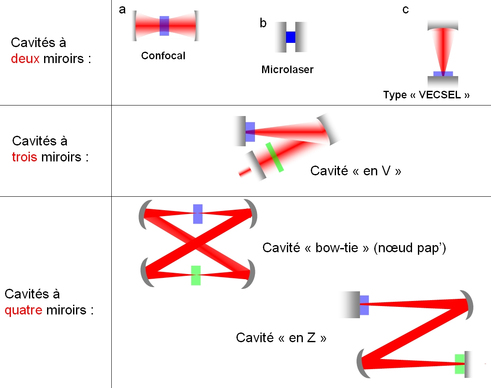
\includegraphics[scale=1.7]{images/fig17.jpg}
\captionof{figure}{ Différents exemples de cavités laser}
\par}

{\centering
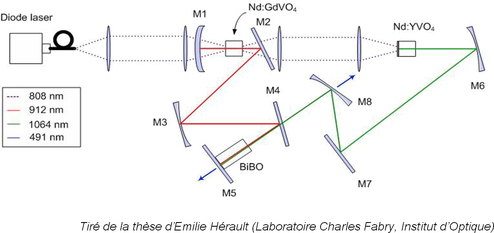
\includegraphics[scale=1.7]{images/fig18.jpg}
\captionof{figure}{ Exemple de cavité laser complexe}
\par}

\section{Les modes d'ordre superieur}
\subsection{Introduction}
Nous avons considéré dans ce qui précède une seule solution de l'équation d'onde paraxiale, à savoir le mode fondamental gaussien. Il existe d'autres solutions, appelées « modes d'ordre supérieur », qui forment une base complète et orthogonale de fonctions. Toute oscillation dans une cavité est une combinaison linéaire de ces modes. La structure transverse de ces modes, de symétrie rectangulaire, cylindrique, ou une combinaison linéaire des deux, est en théorie imposée par la forme des miroirs (rectangulaire ou sphérique). En pratique, de nombreuses perturbations sont susceptibles d'altérer cette structure. 

\subsection{Modes Hermite-Gaussien}


Commençons par nous limiter aux modes relatifs à des coordonnées cartésiennes, liés à une géométrie rectangulaire.

On peut alors écrire une solution de l'équation d'onde sous la forme :
\[\psi(x, y, z) = g\left(\frac xw\right) h\left(\frac yw\right)e^{-i\left(\Delta\phi(z)+\frac
k{2q(z)}(x^2+y^2\right)}\]
où \(g\) (resp. \(h\)) est une fonction de \(z\) et de \(x\) (resp. de \(z\) et de \(y\)).

En intégrant cette solution dans l'équation d'onde paraxiale, on obtient une équation différentielle pour \(g\) et \(h\) qui admet pour solution des polynômes d'Hermite.

On peut montrer (mais on ne le fera pas ici) que l'on obtient un ensemble complet de solutions sous la forme :
\[E_{mn}(x, y, z)=\sqrt{\frac 2\pi \frac 1{2^{m+n}}\frac 1{m!n!}}\frac 1w(z)H_m\left(\frac{\sqrt 2 x}{w(z)}\right)H_n\left(\frac{\sqrt 2 y}{w(z)}\right)e^{-i(kz-\phi(z))}e^{-i\left(\frac k{2q}(x^2+y^2)\right)}\]
où :

\begin{itemize}
    \item \(m, n\) sont des entiers
    \item \(q, R, w\) sont les mêmes que ceux définis pour le mode fondamental gaussien
    \item \(\phi(z)=(m+n+1)arctan\left(\frac {\lambda z}{\pi w_0^2}\right)\)
    \item \(H_m(X)=(-1)^me^{X^2}\frac {\partial ^m}{\partial X^m}e^{X^2}=m!\sum_{p=0}^{\frac m2}\left((-1)^p\frac{(2X)^{m-2p}}{p!(m-2p)!}\right)\) le polynôme d'Hermite d'ordre \(m\)
    \item On a par exemple \(H_0(X) = 1, H_1(X) = 2X, H_2(X) = 4X^2-2\), ...
    \item Pour \(m = n = 0\), on retrouve le mode fondamental gaussien.
    \item Pour \(m\) et \(n\) quelconques, la loi de propagation pour \(R\), \(q\) et \(w\) est inchangée. Seuls le déphasage et la structure transverse du faisceau sont différents.
\end{itemize}

On peut observer sur les figures 19 et 20 la répartition d'intensité pour ces modes. On note la présence de « zéros », sous forme de lignes sombres, dont le nombre correspond à l'ordre considéré.

{\centering
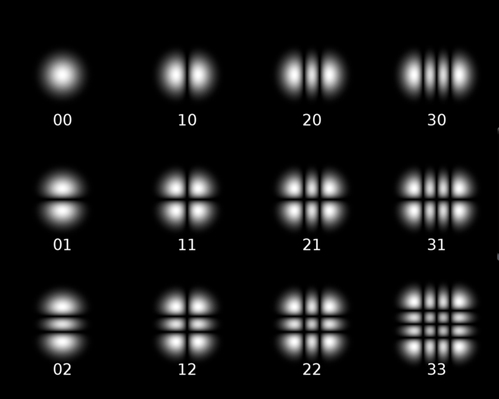
\includegraphics[scale=1.7]{images/fig19.jpg}
\captionof{figure}{Répartition spatiale de l'énergie dans les modes d'ordre supérieur à symétrie rectangulaire (1)}
\par}

{\centering
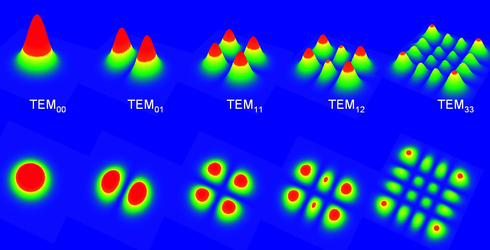
\includegraphics[scale=1.7]{images/fig20.jpg}
\captionof{figure}{ Répartition spatiale de l'énergie dans les modes d'ordre supérieur à symétrie rectangulaire (2)}
\par}

</div>
\paragraph{Spectre de fréquence pour une cavité classique à deux miroirs}
Le déphasage au bout d'un aller-retour dans une cavité à deux miroirs doit être un multiple de \(2\pi\). En partant du terme de phase et en procédant comme au paragraphe intitulé "Fréquence des modes \(TEM_{00}\) dans le cavité" on obtient l'expression de la fréquence d'un mode \(TEM_{mnq}\).
\[\nu_{mnq}=\frac 2{2d}\left(q+\frac 1\pi (m+n+1) arccos(\pm\sqrt{g_1g_2})\right)\]
\(g_i\) est le paramètre \(1-\frac d R_i\) défini pour une cavité de longueur \(d\) et les rayons de courbure des miroirs \(R_i\). Pour \(m=n=0\) on retrouve évidemment l'expression du paragraphe "Fréquence des modes \(TEM_{00}\) dans la cavité" pour le mode fondamental.

Le spectre des fréquences dépend des valeurs des rayons de courbure :

\begin{itemize}
    \item Regardons ce qui se passe pour un résonateur quasi-plan (\(R_1\) et \(R_2\) égaux et très grands devant \(d\)):
\end{itemize}

Le terme en \(arccos\) de l'expression ci-dessus devient \(arccos(g)\) et \(g\) est proche de 1 donc on peut écrire: \(arccos(g)\approx\sqrt\frac {2d}R \ll 1\). Les fréquences \(\nu_{mnq}\) sont très proches des fréquences \(\nu_{00q}\). L'intervalle spectral \(\delta\nu\) pour
\(\Delta m =1\) ou \(\Delta n =1\) vaut \(\frac 1 \pi \sqrt \frac{2d}R\frac c{2d}\) soit quelques dizaines de MHz environ.

\begin{itemize}
    \item Pour une cavité symétrique quasi-confocale (\(R_1 = R_2 = d\)) on trouve un écart entre les modes de \(\frac c{4d}\) et une dégénérescence des fréquences (les modes longitudinaux et certains modes transverses ont la même fréquence).
\end{itemize}

\subsection{Modes Laguerre-Gaussien}

 Si la symétrie de la cavité est plutôt cylindrique, on obtient des modes à symétrie circulaire décrits par des polynômes dit « de Laguerre ». Le traitement est similaire à celui effectué pour les modes Hermite-gaussiens, et nous ne le développerons pas ici. On peut observer sur la figure 21 la répartition d'intensité pour ces modes. 
 
{\centering
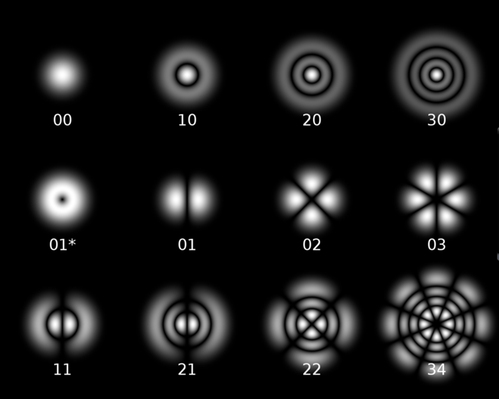
\includegraphics[scale=1.7]{images/fig21.jpg}
\captionof{figure}{ Répartition spatiale de l'énergie dans les modes d'ordre supérieur à symétrie circulaire }
\par}

\subsection{Propagation des faisceaux multimodes et facteur M²}

L'extension radiale des modes d'ordre supérieur est toujours plus importante que celle du mode fondamental d'un facteur constant \(M\). On définit par conséquent:
\[w_{mn}(z)=Mw_{00}z\]
où \(w_{mn}\) et \(w_{00}\) représentent les rayons des faisceaux d'ordre supérieur et fondamental, respectivement.

En injectant cette équation dans la définition du rayon de courbure complexe on obtient :
\[\frac 1{q(z)}=\frac 1{R(z)}-i\frac{M^2\lambda}{\pi w_{mn}^2}\]

On retrouve ensuite toutes les formules démontrées précédemment en remplaçant partout \(\lambda\) par \(M^2\lambda\). Pour \(M^2=1\), on retrouve bien sûr les expressions relatives au mode fondamental.

Le « facteur \(M^2\) » supérieur à 1 mesure donc la « dégradation » de la qualité du faisceau par rapport au mode fondamental pris comme référence.

\textbf{\color{definition1}Définition :}  
\begin{mdframed}[linecolor=definition1, backgroundcolor=definition2]

Plus précisément, \(M^2\) est le facteur par lequel est multiplié l'angle de divergence du faisceau pour un rayon donné :
\[\theta = M^2\frac\lambda{\pi w_0} = M^2\theta_{00}\]
où \(\frac \lambda{\pi w_0}\) est la divergence d'un faisceau gaussien de même waist que le faisceau considéré.

\end{mdframed}


En pratique, il est rare que l'on ait à faire à des modes d'ordre supérieur (on essaie souvent d'avoir un beau faisceau gaussien \(TEM_{00}\)). Pour un faisceau «monolobe», d'allure gaussienne, on mesure le facteur \(M^2\) pour savoir si on est proche ou pas d'un faisceau \(TEM_{00}\) parfait. En d'autres termes, le facteur \(M^2\) donne une
mesure de l'écart à la limite théorique de la diffraction.

Le principe de la mesure est simple : il s'agit de mesurer la divergence et le waist \(w_0\) du faisceau considéré, et de comparer la divergence mesurée avec \(\frac \lambda{\pi w_0}\): le rapport des deux donne la valeur de \(M^2\), et on a ainsi un faisceau « \(M^2\) » fois limité par la diffraction.

Techniquement, on focalise le faisceau à caractériser avec une lentille, puis on mesure avec une méthode adaptée (caméra, mesure d'énergie passant par un diaphragme...) la taille de \(w\) pour différentes positions le long de l'axe \(z\). On obtient une courbe qui ressemble à celle de la figure 11, que l'on ajuste avec la formule donnant \(w(z)\) incluant \(M^2\) comme paramètre d'ajustement.

Les faisceaux sortant des lasers tels que les lasers \(He-Ne\) ou les lasers solides pompés par diode de faible puissance sont généralement limités par la diffraction (\(M^2=1\) ou presque). Les lasers de puissance (par exemples les lasers \(Nd:YAG\) pompés par flash) ont souvent une structure transverse hétérogène et le facteur \(M^2\) grimpe jusqu'à quelques unités. Il se peut également qu'il soit différent suivant le choix des axes \(x\) et \(y\).
Enfin pour des faisceaux non-gaussiens, comme ceux sortant des diodes lasers de puissance, on peut avoir des \(M^2\) de plusieurs dizaines d'unités: la signification physique du paramètre \(M^2\) dans ce cas est néanmoins discutable.

\section{Conclusion}
L'étude des cavités est un préalable indispensable à toute construction de laser. Dans ce cours, nous n'avons abordé que les structures passives simples : pour des architectures plus complexes, il existe de nombreux logiciels sur le marché permettant de simuler toutes sortes de cavités laser. Dans certains, il est également possible de prendre en compte les effets que nous avons négligés ou passé sous silence ici :
\begin{itemize}[label=\textbullet]
    \item Influence de la taille finie des miroirs : la diffraction joue alors un rôle important si les miroirs sont de dimensions très faibles. Le facteur intéressant dans ce cadre est le nombre de Fresnel $N=\frac{a_1a_2}{\lambda d}$ où $a_1$ et $a_2$ sont les rayons (pas les rayons de courbure !) des miroirs de la cavité. Si $N \gg 1$, la diffraction est négligeable.
    \item Astigmatisme pour les systèmes non-centrés ou comportant des miroirs utilisés hors d'axe (comme les cavités en V par exemple).
    \item Effets liés à la cavité active, c'est à dire à la présence du milieu amplificateur pompé qui s'échauffe, se déforme...
    \item Effets de la polarisation
\end{itemize}

Pour compléter ce cours, vous pouvez consulter les références données en bibliographie.
    
``I always thought something was fundamentally wrong with the universe'' \citep{adams1995hitchhiker} \citep{anthoTropCho} \citep{herwigLaser} \citep{laguerreDesEtoiles}

\chapter{Étude de cas}
\section{Introduction}

L'objectif de cette étude est d'étudier concrètement une cavité laser telle que celle utilisée dans l'étude de cas du grain «laser – principes de base». Cette étude permet de mettre en application les notions exposées dans le cours de façon concrète.

Rappelons la géométrie utilisée (voir l'étude de cas du grain « laser – principes de base » pour les détails) et définissons les différentes grandeurs dont nous aurons besoin pour l'étude :

\begin{itemize}
    \item un cristal de Nd:YAG de longueur \(l\)=10 mm et d'indice \(n=1,8\) est utilisé comme milieu amplificateur dans une cavité linéaire à deux miroirs.
    \item L'un des deux miroirs est déposé directement sur une des face du cristal (il est donc plan) : ce miroir doit être transparent à la longueur d'onde de pompe (808 nm) et hautement réfléchissant à la longueur d'onde laser (on notera \(A1\) son coefficient de réflexion à 1064 nm : il est proche de 1) : il est composé d'une succession de couches sub-micrométriques de matériaux de haut et bas indice respectivement. Avec cette technique, quasiment tous les profils spectraux de réflectivité sont potentiellement réalisables.
    \item L'autre miroir, de rayon de courbure \(R\), ferme la cavité : il laisse passer un pourcentage donné de lumière à 1064 nm pour constituer le faisceau laser. On notera \(A2\) son coefficient de réflexion à 1064 nm.
    \item La distance physique entre la face non traitée du cristal et le miroir de sortie sera notée \(L\) (qui n'est donc pas ici la largeur du fleuve. La longueur totale de la cavité est donc égale à \(L+l\).
\end{itemize}

{\centering
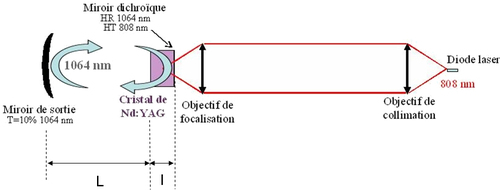
\includegraphics[scale=1.7]{images/EC_Fig1.jpg}
\captionof{figure}{Schéma global du laser}
\par}

\section{Étude préliminaire de la cavité hémisphérique}
\subsection{Stabilité de la cavité}

Écrivons la matrice ABCD sur un aller retour :

en observant la figure 2, le trajet aller-retour se décompose en :

\begin{itemize}
    \item le parcours d'une distance \(L\) dans l'air
    \item le parcours d'une distance \(l\) dans le cristal d'indice \(n\)
    \item la réflexion sur un miroir plan, qui n'a aucune incidence
    \item à nouveau les parcours sur la distance \(l\) dans le cristal puis \(L\) dans l'air
    \item enfin la réflexion sur le miroir de rayon de courbure \(R\).
\end{itemize}

{\centering
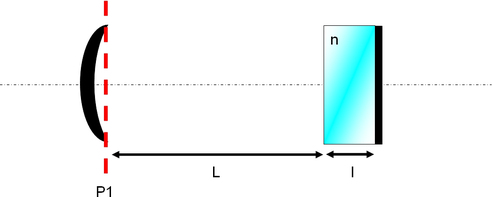
\includegraphics[scale=1.7]{images/EC_Fig2.jpg}
\captionof{figure}{Schéma de la cavité}
\par}

La cavité dépliée est représentée sur la figure 3 et correspond à la suite de matrices suivantes (attention à l'ordre !):
\[T=\begin{pmatrix}
1 & 0 \\
-\frac 2R & 1
\end{pmatrix}\begin{pmatrix}
1 & L \\
0 & 1
\end{pmatrix}\begin{pmatrix}
1 & \frac ln \\
0 & 1
\end{pmatrix}\begin{pmatrix}
1 & \frac ln \\
0 & 1
\end{pmatrix}\begin{pmatrix}
1 & L \\
0 & 1
\end{pmatrix}\]

{\centering
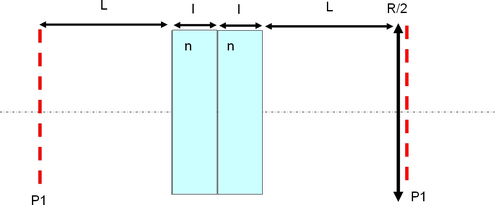
\includegraphics[scale=1.7]{images/EC_Fig3.jpg}
\captionof{figure}{ Cavité dépliée}
\par}

En posant \(d = L + \frac ln\) pour alléger les notations, on trouve après calcul:
\[T = \begin{pmatrix}
1 & 2d \\
-\frac 2R & 1-\frac {4d}R
\end{pmatrix}\]

Pour que la cavité soit stable, il faut que \(0 < \frac{A+D+2}4 < 1\) ce qui se résume ici à: \(0 < 1-\frac d R < 1\), soit une simple condition à vérifier (puisque \(\frac dR\) est évidemment positif):

\(d < R\) soit en reprenant les notations de base \(L < R-\frac ln\)

\textbf{\color{remarque1}Remarque :}  
\begin{mdframed}[linecolor=remarque1, backgroundcolor=remarque2]

Pour une cavité « vide », sans cristal, de longueur \(L_{eq}\), la condition de stabilité se serait écrite (voir cours): \(0 < g_1g_2 < 1\) or \(g_1=1-\frac {L_{eq}}{R_{plan}}=1\) car \(R_plan\) est infini (miroir plan), donc la condition devient \(g_2=1-\frac{L_{eq}}R > 0\) ou encore \(L_{eq} < R\).

La cavité avec le cristal est donc équivalente du point de vue de la stabilité à une cavité vide de longueur équivalente \(L_{eq}=d=L+\frac ln\).

\end{mdframed}

\textbf{\color{attention1}Attention :}  
\begin{mdframed}[linecolor=attention1, backgroundcolor=attention2]

Il est facile de se tromper en prenant comme longueur équivalente la longueur optique \(L+nl\) !

\end{mdframed}


Revenons à notre cavité: on peut donc choisir n'importe quel couple (rayon de courbure \(R\) – Distance \(L\)) vérifiant la condition \(L < R-\frac ln\). En pratique, on verra que d'autres considérations, comme la taille souhaitée du waist dans la cavité, peuvent influer sur ces choix. De plus, on ne dispose pas concrètement d'un nombre illimité de miroirs de rayons de courbures différents !

Pour l'instant, prenons un miroir de rayon \(R\) = 100 mm.

La longueur \(L\) doit donc être inférieure à \(100-\frac {10}{1,8} \approx\) 94,5 mm.

On prendra pour fixer les idées dans la suite \(L\) = 80 mm.

\subsection{}

Maintenant que les dimensions permettant de stabiliser la cavité ont été choisies, regardons de plus près à quoi va ressembler le faisceau dans la cavité.

On sait déjà que le \textbf{\color{red}waist va se situer au niveau du miroir plan}, puisque le faisceau doit revenir sur lui-même.

Commençons par déterminer la taille des faisceaux sur les miroirs, que l'on notera \(w_0\) sur le miroir plan et \(w_1\) sur le miroir sphérique, ainsi que la divergence et la longueur de Rayleigh \(Z_R\) associées :

On va raisonner pour simplifier sur la cavité équivalente de longueur \(L_{eq}=d=L+\frac ln\).

En prenant \(z=0\) au niveau du miroir plan, on peut écrire qu'en \(z = d\), c'est à dire sur le miroir sphérique, le rayon de courbure du faisceau laser doit être le même que celui du miroir (toujours pour assurer un retour sur lui-même du faisceau). Or on connaît la loi de variation de \(R\) avec \(z\) (voir cours), ce qui nous amène à écrire :
\[R=R(z=d)=d\left(1+\left(\frac{\pi w_0^2}{\lambda d}\right)^2\right)= d\left(1+\left(\frac{Z_R}d\right)^2\right)\]
on en déduit facilement
\[Z_R=\sqrt{d(R-d)}=\frac {\pi w_0^2}\lambda\]
avec \(d = L+\frac ln = 80+\frac {10}{1,8}\) = 85,5 mm et \(R\) = 100 mm il vient: \(Z_R\) = 35,2 mm et \(w_0\) = 110 µm (la longueur d'onde vaut 1064 nm)

La divergence vaut \(\theta = \frac \lambda {\pi w_0}\) soit 3 mrad.

Pour connaître le rayon du faisceau sur le miroir sphérique, on applique simplement la formule suivante :
\[w(z)=w_0\sqrt{1+\left(\frac {\lambda z}{\pi w_0^2}\right)^2}\]
ce qui nous donne en \(z=d\) :
\[w_1=\sqrt{\frac {\lambda R}\pi} \sqrt[4]{\frac d{R-d}}\]
soit numériquement \(w_1\) = 286 µm.

La structure du faisceau dans la cavité est donc la suivante (figure 4):

{\centering
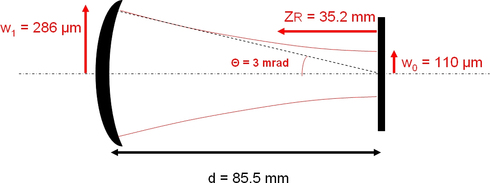
\includegraphics[scale=1.7]{images/EC_Fig4.jpg}
\captionof{figure}{ Caractéristiques du faisceau laser dans la cavité}
\par}

\section{Cavité réelle}
\subsection{Optimisation de la cavité}


Nous avons déterminé la géométrie du faisceau pour une longueur \(L\) fixée arbitrairement.

En pratique, cette géométrie est fixée par des conditions extérieures, notamment liées au pompage de la cavité. On a vu par exemple (voir étude de cas du grain « principes de base du laser ») que la géométrie de pompage conduisait à un rayon du faisceau de pompe fixé. Dans le cas précis décrit, le faisceau de pompe se focalise sur un ovale de dimension 20 x 100 µm en raison de l'utilisation d'une barrette de diodes laser 1 x 100 µm comme \(\Delta \nu\) pompe. Pour simplifier ici les calculs, nous supposerons que le pompage est circulaire (par exemple en utilisant une pompe fibrée), de rayon 80µm dans le cristal après passage dans les optiques de collimation/focalisation.

Il est important que le mode laser et le mode de pompe soient bien adaptés : on va donc chercher à obtenir un mode laser qui soit compatible avec la dimension du faisceau de pompe dans le cristal. Plus précisément, on va choisir de prendre un mode laser légèrement plus petit que le mode de pompe, afin d'avoir une pompe bien homogène sur toute la surface du mode de cavité.

On va donc chercher à avoir disons \(w_0\) = 60 µm.

\textbf{\color{remarque1}Remarque :}  
\begin{mdframed}[linecolor=remarque1, backgroundcolor=remarque2]

On peut faire une analyse plus poussée pour déterminer quelle est la taille optimale du mode pour une géométrie de pompage donnée, mais cela est au-delà de ce cours.

\end{mdframed}

Quelle est la longueur \(L\) à choisir dans ce cas, en utilisant toujours notre miroir \(R\) = 100 mm ?

Reprenons la formule \(Z_R=\sqrt{d(R-d)}=\frac{\pi w_0^2}\lambda\); on obtient un trinôme en \(d\):

\(d^2-dR+\left(\frac{\pi w_0^2}\lambda \right) ^2=0\) dont la résolution mène à deux valeurs de \(d\):

\(d_1\) = 98,85 mm et \(d_2\) = 1,14 mm.

Bien sûr seule la première conduit à une valeur ayant un sens physique (pour la seconde, \(L\) est négatif) et donne \(L\) = 93,3 mm.

On est toujours dans la zone de stabilité, mais en limite de cette dernière.

On peut tracer (figure 5) l'évolution de la taille du waist avec \(L\) pour une valeur donnée de \(R\) (ici 100 mm). Bien sûr pour \(L > R\) la cavité n'est plus stable et le waist n'a pas de sens.

On voit qu'il existe une zone où le waist garde une taille stable, pour \(L\) autour de \(\frac R2\) = 50 mm. On observe également qu'avec notre miroir de rayon 100 mm, il est impossible d'avoir un waist supérieur à 130 µm. Par contre on peut obtenir des waists très petits en flirtant avec la limite de stabilité.

{\centering
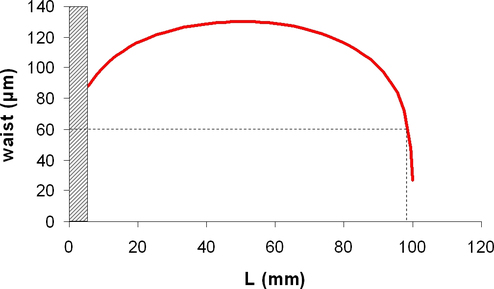
\includegraphics[scale=1.7]{images/EC_Fig5.jpg}
\captionof{figure}{ Evolution du waist avec L}
\par}

\subsection{Faisceau en sortie}


A quoi va ressembler le faisceau à la sortie du laser, à travers le miroir sphérique ?

Ce miroir est partiellement transparent, et possède une face sphérique concave (c'est la face utile pour la cavité) et une face plane (l'arrière du substrat sur lequel est déposé le miroir).

{\centering
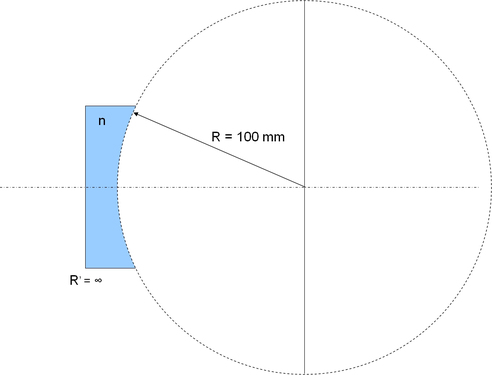
\includegraphics[scale=1.7]{images/EC_Fig6.jpg}
\captionof{figure}{ Miroir de sortie}
\par}

Le miroir de sortie se comporte donc vis-à vis du faisceau laser sortant comme une lentille divergente.

Sa focale \(f'\) est donnée par la « formule des opticiens » (voir cours d'optique géométrique) :

\(\frac 1 {f'}=(n_M-1)\left(\frac 1{R'}-\frac 1R\right)\) avec \(R'\) = rayon de la face plane = \(\infty\) et \(n_M\) l'indice du substrat sur lequel est déposé le miroir.

On a donc \(f'=\frac R {1-n_M}\), soit numériquement en prenant \(n_M\) = 1,5 (verre): \(f'\) = -200 mm.

On a déjà déterminé la divergence du faisceau dans la cavité. Combien vaut-elle maintenant en dehors ?

On va chercher le nouveau rayon de courbure complexe après le miroir de sortie, soit après une lentille divergente de focale \(f'\). Pour cela, on applique la loi ABCD :

\(q(apres)=\frac{Aq(avant)+B}{Cq(avant)+D}\) en notant \(q(avant)\) le rayon de courbure complexe avant traversée du miroir de sortie et \(q(apres)\) le rayon de
courbure complexe après traversée de ce même miroir.

Les coefficients ABCD sont ceux de la matrice de transfert d'une lentille :
\[T= \begin{pmatrix}
1 & 0 \\
-\frac 1f & 1
\end{pmatrix}\]

On en déduit que :
\[\frac 1{q(apres)}=\frac 1{q(avant)}-\frac 1{f'}\]

NB : c'est une formule utile dans bien des cas lorsque l'on transforme un faisceau gaussien via une lentille.

On a également \(\frac 1{q(avant)}=\frac 1R-i\frac \lambda{\pi w_1^2}\) et \(\frac 1{q(apres)}=\frac 1{R'}-i\frac \lambda{\pi w_1^2}\) (la taille du faisceau ne change pas entre les deux faces de la lentille dans l'hypothèse « lentille mince »).

On en déduit que par identification que \(R'=\frac R{n_M}\).

En utilisant la formule du cours :
\[w_0^2 = \frac {w^2}{1+\left(\frac{\pi w^2}{\lambda R}\right)^2}\]
avec la nouvelle valeur de R', on trouve le « waist effectif » pour le faisceau sortant de la cavité:
\[w_0'^2 = \frac {w_1^2}{1+\left(\frac{\pi w_1^2n_M}{\lambda R}\right)^2}\]

En remplaçant \(w_1\) par sa valeur en fonction de \(w_0\) trouvée précédemment, soit \(w_1=\sqrt{\frac{\lambda R}{\pi}}\sqrt[4]{\frac d{R-d}}\) on trouve:
\[w_0'^2 = \frac {w_1^2}{1+\left(\frac{dn_M^2}{R-d}\right)}\]

Comme de plus \(w_1=w_0\sqrt{1+\frac {d^2}{Z_R^2}}\) et \(Z_R=\sqrt{d(R-d)}\) on en déduit:
\[w_0'^2=\frac {R w_0^2}{R+(n_M^2-1)d}\]

On en déduit la nouvelle divergence \(\theta '\):
\[\frac {\theta '}\theta = \frac{w_0}{w'_0}=\sqrt{1+(n_M^2-1)\frac dR}\]

Numériquement, la nouvelle divergence vaut 1,438 fois celle avant le passage par le miroir de sortie (on a pris ici les valeurs pour \(d\)=85,5 mm – voir figure 4) soit 4,3 mrad.

\subsection{Effet de lentille thermique}

Rapprochons nous encore de la réalité : la pompe dépose une grande quantité d'énergie sur une petite surface dans le cristal. Il en résulte un échauffement local, et donc comme l'indice de réfraction varie avec la température un gradient d'indice apparaît. D'autre part, la dilatation thermique du cristal induit un « bombement » de ces faces. Ce deuxième effet est responsable de la transformation du miroir plan déposé sur le cristal en un miroir concave.

L'effet de gradient d'indice peut être en première approximation modélisé par l'ajout d'une lentille mince équivalente au niveau du point de focalisation de la pompe dans le cristal.

Nous n'effectuerons pas ici les calculs qui s'avèrent fastidieux à effectuer « à la main », cependant le principe est simple puisqu'il s'agit juste de rajouter des éléments dans la cavité. Ce type de calcul est très facilement géré par ordinateur (il s'agit de simples multiplications de matrices) et plusieurs logiciels spécialisés existent sur le marché.

On se rapproche ainsi de la cavité réelle et l'on peut ainsi modéliser assez finement les caractéristiques géométriques du faisceau laser. 

\section{Modes longitudinaux}


Nous allons pour terminer déterminer les fréquences des modes longitudinaux de la cavité : le déphasage subi par l'onde sur un aller simple dans la cavité est égal à (voir cours):
\[\Delta \phi = \phi (d) = \phi (0) = -k(D) + \zeta (d) - \zeta (0) = -q\pi\]
avec \(k=2\pi \frac \nu c\), \(D\) le chemin optique parcouru \((D=L+nl)\), \(tan(\zeta(0))=0\), et \(tan(\zeta(d))=\frac d {Z_R} = \sqrt\frac d{R-d}\) .

Par conséquent :
\[\nu _q = \frac c {2D} \left( q+\frac 1 \pi \left( arctan\left(\sqrt\frac d {R-d}\right)\right)\right)\]
et pour les modes transverses :
\[\nu _{mnq} = \frac c {2D} \left( q+\frac {m+n+1} \pi \left( arctan\left(\sqrt\frac d {R-d}\right)\right)\right)\]

On trouve en prenant \(L\) = 80 mm un écart entre deux modes longitudinaux de l'ordre de 1,5 GHz et un écart entre le mode fondamental et le premier mode transverse de 575 MHz (voir figure 7).

\textbf{\color{remarque1}Remarque :}  
\begin{mdframed}[linecolor=remarque1, backgroundcolor=remarque2]

Pour que la longueur d'onde (1064 nm) corresponde à la fréquence relative à l'ordre \(q\), il faut que \(q\) vaille environ \(1,195.10^8\).

{\centering
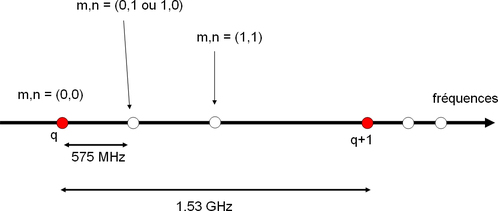
\includegraphics[scale=1.7]{images/EC_Fig7.jpg}
\captionof{figure}{Position des modes longitudinaux}
\par}

\end{mdframed}

\chapter{Exercices}

\section{Énoncés}
\subsection{Transformation de faisceau laser}
On cherche à focaliser un faisceau laser collimaté, issu d'un laser \(He-Ne\) (longueur d'onde = 633 nm), de taille \(w\) = 1 mm, situé à une position \(z=0\) de telle façon que la longueur de Rayleigh du faisceau focalisé soit égale à 30 mm.
\paragraph{Question:}
Quelle distance focale doit posséder la lentille qu'il faut utiliser ?

\subsection{Caractéristique d'un faisceau laser}
La condition de stabilité pour une cavité à deux miroirs est:
\[0 < g_1g_2 < 1\]
avec ici \(g_1=1-\frac d{R_{plan}}; g_2=1-\frac dR\).

La condition devient donc \(d < R\) ce qui est toujours vérifié car \(R=2d\).

\paragraph{Question 1:}
Montrez que cette cavité est stable. 
\paragraph{Question 2:}
Déterminez les caractéristiques géométriques du faisceau laser dans la cavité (waists sur les miroirs, longueur de Rayleigh, divergence).

\subsection{Stabilité}
Un résonateur est constitué de deux miroirs, un concave et un convexe, de rayons respectifs 1,5 m et -1 m. La distance qui les sépare est $d$. 
\paragraph{Question:}
Combien peut-elle valoir pour que la cavité soit stable ? 

\subsection{Énergie}
Soit un faisceau gaussien de rayon . 
\paragraph{Question:}
Quel pourcentage de l'énergie de ce rayon est transmis à travers un diaphragme circulaire de rayon $\rho$, centré sur le faisceau ?

Application numérique pour: $\rho=0.5w; \rho = 0.75w; \rho=w; \rho = 2w$

\subsection{Répartition spectrale des modes longitudinaux}
On dispose d'un laser Hélium-Néon, de longueur optique de cavité égale à 20 cm et émettant à 632,8 nm. 
\paragraph{Question 1:}
Quel est l'écart, en fréquence et en longueur d'onde, entre deux modes longitudinaux consécutifs ? 
\paragraph{Question 2:}
On dispose d'un filtre spectral de bande passante 1 nm. De combien faut-il modifier la longueur de la cavité laser pour pouvoir grâce à ce filtre sélectionner un unique mode longitudinal ? 


\section{Correction}

\subsection{Transformation de faisceau laser}
On veut $Z_R=\frac {\pi w'^2}{\lambda}$ = 30 mm soit pour une longueur d'onde de 633 nm : $w'$= 78µm

On sait que dans ce cas (« infini-foyer », c'est à dire que l'un des waists est au foyer de la lentille – et donc l'autre aussi par voie de conséquence) $w' = \frac {\lambda f}{\pi w}$

Donc 
$$f=\frac{\pi w w'}\lambda = 387mm$$

\subsection{Caractéristique d'un faisceau laser}

\paragraph{1)}
La condition de stabilité pour une cavité à deux miroirs est:
$$0 < g_1g_2 < 1$$
avec ici $g_1=1-\frac d{R_{plan}}; g_2=1-\frac dR$
La condition devient donc $d < R$ ce qui est toujours vérifié car $R=2d$.

\paragraph{2)}
$$R=2d=d\left(1+\frac{Z_R^2}{d^2}\right)$$
puisque le rayon du front d'onde doit être égal au rayon de courbure du miroir sur celui ci. 
 
Par suite $\theta=\frac\lambda{\pi w_0}$; $w_0=\sqrt{\lambda\frac d \pi}$ et $\theta=\frac\lambda{\pi w_0}$

\subsection{Stabilité}

Pour une cavité à deux miroirs, la condition de stabilité s'écrit: $0 < g_1g_2 < 1$

Ce qui se réécrit $0 > (R_1-d)(R_2-d) > R_1R_2$

Finalement après résolution du trinôme, on trouve que $d$ doit être compris entre 0.5 et 1.5 m (exclus).

\subsection{Énergie}

Le profil d'intensité d'une gaussienne est :
\[I(r, z) = I_0(z) e^\frac{-2r^2}{w^2(z)}\]
et \(r\) va de 0 à l'infini.

Par une ouverture de rayon \(r\), il passe donc une fraction \(F\) de l'énergie définie par:
\[F=\frac{\int_0^\rho I(r) dS}{\int_0^\infty I(r) dS}\]
avec \(dS=2\pi r dr\)

En remplaçant \(I(r)\) par sa valeur à un point \(z\) donné (correspondant à une valeur \(w\) de \(w(z)\), il vient après simplification:
\[F=\frac{\int_0^\rho re^\frac{-2r^2}{w^2} dr}{\int_0^\infty re^\frac{-2r^2}{w^2} dr}\]

Un simple changement de variable (en posant \(t=r^2\)) permet de calculer cette intégrale:
\[\int_0^\rho re^\frac{-2r^2}{w^2} dr = \frac 12 \int_0^{\rho ^2} e^\frac{-2t}{w^2} dt = \frac 12 \left[\frac {-w^2}2e^\frac{-2t}{w^2}\right]_0^{\rho ^2}\]


Finalement on trouve :
\[F = 1-e^{-2\left(\frac rw\right)^2}\]
soit pour les applications numériques, on a respectivement les résultats suivants:

\begin{itemize}
    \item pour \(\frac rw\) = 0.5 on a \(F\) = 0.39
    \item pour \(\frac rw\) = 0.75 on a \(F\) = 0.67
    \item pour \(\frac rw\) = 1 on a \(F\) = 0.86
    \item pour \(\frac rw\) = 2 on a \(F\) = 0.999
\end{itemize}

\textbf{\color{remarque1}Complément :}  
\begin{mdframed}[linecolor=remarque1, backgroundcolor=remarque2]

Si le rayon du diaphragme vaut celui du faisceau, seule 86\% de l'énergie est transmise. Cela est dû au fait que le rayon \(w\) représente la largeur du faisceau laser à \(\frac 1{e^2}\): toute l'énergie comprise dans « les ailes » de la gaussienne (\(r > w\)) est donc perdue avec ce diaphragme.

On voit aussi avec cette application numérique qu'il faut un diaphragme deux fois plus grand que le faisceau (toujours défini par \(w\)) pour récupérer toute l'énergie.

\end{mdframed}

\subsection{Répartition spectrale des modes longitudinaux}

\paragraph{1)}
\[\Delta \nu_q = \frac c {2L} = \frac {3\times 10^8}{0.4} = 750MHz\] 
\(\frac {\Delta \lambda}{\lambda} = \frac {\Delta \nu}{\nu}\) donc \(\Delta \lambda\) = 1 pm
            
La condition devient donc \(d < R\) ce qui est toujours vérifié car \(R=2d\).
\paragraph{2)}
On veut pour le laser \(He-Ne\) que \(\Delta \lambda > 0.5nm\) ou encore \(\Delta \nu = \frac{c\Delta\lambda}{\lambda ^2} > 3.75\times 10^{11} Hz\).

On en déduit qu'il faut que \(L < 0,4 mm\).


\bibliographystyle{plain}
\bibliography{references}
\end{document}
